\chapter{Real Data}
\label{sec:RealData}
The ultimate goal of modeling the BOLD response is to estimate parameters
in real FMRI data. The most basic use of modeling the BOLD signal is to
locate activation. A voxel is considered active when the stimulus 
is the primary drive for the BOLD response. This is in contrast to 
most voxels which have are controlled by intermediate or complete unrelated factors. 
Inactive regions cannot be modeled because their input is unknown, therefore
parameter estimates in such regions are impossible. 
Because SPM is the de facto standard for localizing activation,
this section compares its output with that of the particle filter.

Note that SPM must pre-process the image with a spatial smoothing 
filter. For this work SPM8 was smoothed with a
$8\text{mm} \times  8\text{mm} \times 8\text{mm}$ Full-Width Half Maximum
(FWHM) Gaussian kernel. 
Additionally, SPM8 applied a high pass filter (with a cut
off based on a globally estimated autocorrelation). Thus the preprocessing pipeline
of SPM is very different from that of the particle filter. SPM8 also outputs
a T-statistic for each voxel, whereas the 
particle filter's primary output is a posterior probability distribution of the parameters
at every voxel. To validate the quality of the particle filter, the results 
were compared with SPM, both in terms of the location and the fit.

%scanner info?
\section{Experiment Configuration}
\label{sec:ExperimentConfig}
For the FMRI data discussed in \autoref{sec:RealData}, tests were 
performed on a right handed volunteer using a GE SIGNA HDx 1.5 Tesla
scanner with a single echo EPI sequence. Slice spacing was
5mm, and pixel sizes were 3.75mm.  Repitition Time was 2.1s, 
Echo Time was 40 ms and the imaging frequency was set to $63.854$MHz.
The image resolution was $64 \times 64 \times 28$. 
The subject was presented with either a single or
double flash and was asked to respond with a right handed
or lefted handed finger tap, respectively. The FMRI began 18.9 seconds
before the beginning of the experiment, to allow for transients 
in to image to settle out. The timing of the flashes are shown 
below with time 0 corresponding to the beginning of
the 10th TR (so 9 images were dropped). 

The timing of the single flashes were:

1.706, 11.944, 17.063, 18.769, 34.125, 39.244, 44.231, 47.644, 49.350, 
61.294, 64.706, 66.413, 69.825, 71.531, 73.238, 76.650, 80.063, 
90.169, 96.994, 110.644, 117.469, 120.881, 130.988, 132.694, 154.875, 
158.288, 161.700, 165.113, 168.525, 176.925, 178.631, 183.750, 190.575, 
204.225, 205.931, 211.050, 216.038, 222.863, 226.275, 236.513, 248.456, 
255.281, 258.563, 263.681, 273.919, 277.331, 287.569, 292.688, 294.394, 
299.381

and the timing of the double flashes were:

0.131, 6.825, 20.475, 27.300, 35.831, 52.763, 54.469, 59.588, 86.756, 
91.875, 107.231, 108.938, 112.350, 114.056, 115.763, 119.175, 126.000, 
134.400, 136.106, 141.225, 144.638, 156.581, 159.994, 166.819, 171.806, 
175.219, 185.456, 188.869, 202.519, 212.756, 217.744, 221.156, 227.981, 
229.688, 233.100, 243.338, 245.044, 246.750, 250.163, 261.975, 270.506, 
272.213, 280.744, 282.450, 289.275, 296.100, 301.088, 304.500

%spm options
After dropping the first 9 volumes, each of the remaining volumes was
co-registered with the first. At this point the SPM method
diverges from the experimental method. For the particle filter, detrending 
was then applied as discussed in \autoref{sec:Detrend} and the resulting
data was processed with the particle filter. To generate the SPM output
in this section, the co-registered data was spatially smoothed,
and then filtered with an adaptive cut off (which is built into the
SPM analysis). For the SPM analysis, the Canonical HRF was used
and model time derivatives were included although not in the contrast
vector. All other settings used in SPM8 were left at default
for analyzing FMRI data.

\section{Results}
The results from T-values from SPM8 are shown in \autoref{fig:hm_canon_spm} (threshold of
4), and the results from 
the particle filter are shown in \autoref{fig:hm_canon_pfilter} and \autoref{fig:hm_canon_pfilter_mi}.
Note that the scales for all three images are different, because the metrics are different.
SPM measures using T-Tests to determine the likelihood of a false positive. \autoref{fig:hm_canon_pfilter}
uses simple normalized residuals, meaning that lower indicates less error.  
\autoref{fig:hm_canon_pfilter_mi} measures in terms of the dependence between the 
measured signal and the estimated signal; thus higher indicates a better fit. The particle
filter data shows a large number of false positives, however application of a threshold
of $.85$ on the residual map removes these false positives. Similarly, in the mutual information
map, the false positives may be elminated by upping the threshold to $.15$. However, just
because the results disagree with SPM does not necessarily mean they are false positives.
SPM operates on smoothed data (8mm x 8mm x 8mm), so there are certainly active 
areas that have been missed because of the smoothing. 

\begin{figure}[H]
\subfigure[]{\label{fig:hm_spm} 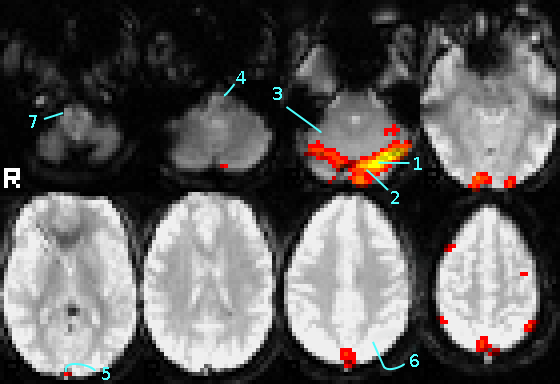
\includegraphics[scale=.85]{images/spm_hm}}
\subfigure[]{\label{fig:hm_canon_spm_x} 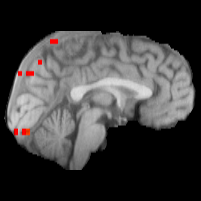
\includegraphics[scale=3]{images/spm_hm_x}}
\subfigure[]{\label{fig:hm_canon_spm_y} 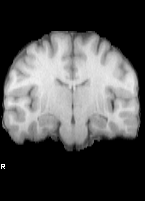
\includegraphics[scale=3]{images/spm_hm_y}}
\subfigure[]{\label{fig:hm_canon_spm_z} 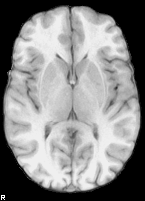
\includegraphics[scale=3]{images/spm_hm_z}}
\subfigure{\label{fig:scale_spm} 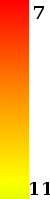
\includegraphics[scale=.5]{images/scale1}}
\caption{SPM results. Units of activation are in Student's T-scores; higher indicates higher 
        assurance that the signal cannot have occurred through noise alone. 
        Sagittal, coronal and axial slices  are 
        \autoref{fig:hm_canon_spm_x}, \autoref{fig:hm_canon_spm_y}, and
         \autoref{fig:hm_canon_spm_z}, respectively. A series of axial slices are
         shown in \autoref{fig:hm_spm}. }
\label{fig:hm_canon_spm}
\end{figure}

\begin{figure}[H]
\subfigure[]{\label{fig:hm_pfilter} 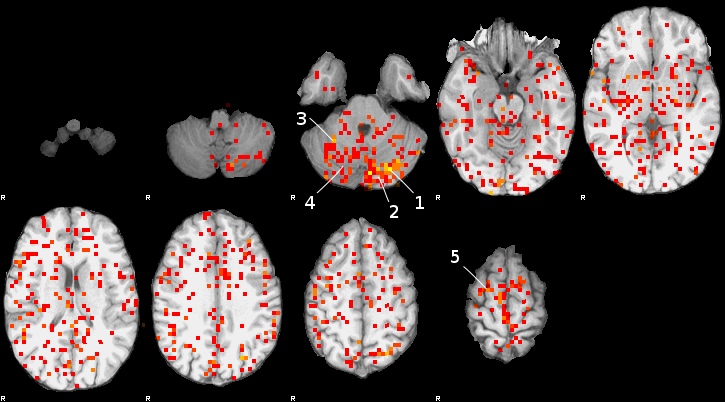
\includegraphics[scale=.85]{images/pfilter_hm}}
\subfigure[]{\label{fig:hm_canon_pfilter_x} 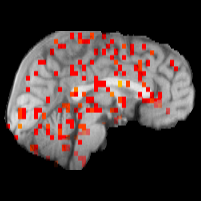
\includegraphics[scale=3]{images/pfilter_hm_x}}
\subfigure[]{\label{fig:hm_canon_pfilter_y} 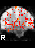
\includegraphics[scale=3]{images/pfilter_hm_y}}
\subfigure[]{\label{fig:hm_canon_pfilter_z} 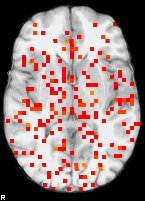
\includegraphics[scale=3]{images/pfilter_hm_z}}
\subfigure{\label{fig:scale_pfilter} 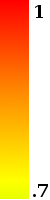
\includegraphics[scale=.5]{images/scale2}}
\caption{Particle Filter results measured in normalized $\sqrt{MSE}$. 
        Units of match is normalized residual where the  the lowest (best) levels shown are
        $.7$ and the highest error shown (threshold) is $1$.
        Sagittal, coronal and axial slices are shwon in \autoref{fig:hm_canon_pfilter_x},
        \autoref{fig:hm_canon_pfilter_y}, and 
         \autoref{fig:hm_canon_pfilter_z}, respectively. A series of axial slices are shown in
         \autoref{fig:hm_pfilter}.  }
\label{fig:hm_canon_pfilter}
\end{figure}

%\begin{figure}[H]
%\subfigure[]{\label{fig:hm_pfilter85} 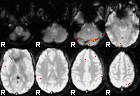
\includegraphics[scale=.75]{images/pfilter85_hm}}
%\subfigure[]{\label{fig:hm_canon_pfilter85_x} 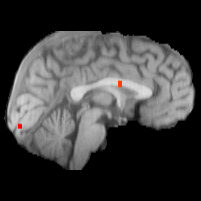
\includegraphics[scale=3]{images/pfilter_hm85_x}}
%\subfigure[]{\label{fig:hm_canon_pfilter85_y} 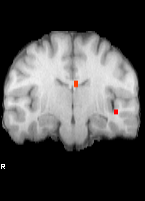
\includegraphics[scale=3]{images/pfilter_hm85_y}}
%\subfigure[]{\label{fig:hm_canon_pfilter85_z} 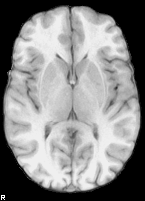
\includegraphics[scale=3]{images/pfilter_hm85_z}}
%\subfigure{\label{fig:scale_pfilter85} 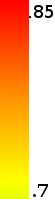
\includegraphics[scale=.5]{images/scale3}}
%\caption{Sagittal, coronal and axial (\autoref{fig:hm_canon_pfilter_x} \autoref{fig:hm_canon_pfilter_y} 
%         \autoref{fig:hm_canon_pfilter_x}), as well as a series of axial slices, \autoref{fig:hm_pfilter}. 
%         Units of match is normalized residual. The lowest (best) levels were $.7$.
%         The highest error shown is $.85$.}
%\label{fig:hm_canon_pfilter85}
%\end{figure}

\begin{figure}[H]
\subfigure[]{\label{fig:hm_mi} 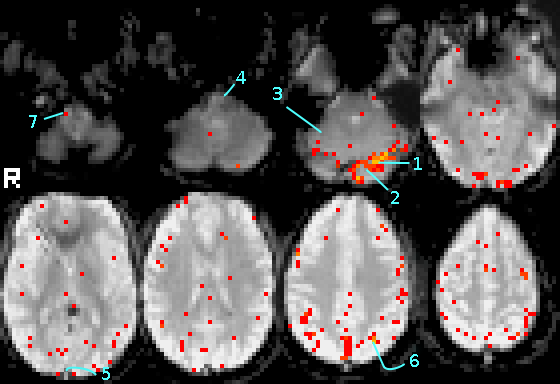
\includegraphics[scale=.85]{images/mi_hm}}
\subfigure[]{\label{fig:hm_canon_mi_x} 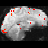
\includegraphics[scale=3]{images/mi_hm_x}}
\subfigure[]{\label{fig:hm_canon_mi_y} 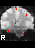
\includegraphics[scale=3]{images/mi_hm_y}}
\subfigure[]{\label{fig:hm_canon_mi_z} 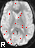
\includegraphics[scale=3]{images/mi_hm_z}}
\subfigure{\label{fig:scale_mi} 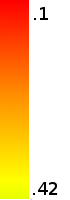
\includegraphics[scale=.5]{images/scale4}}
\caption{Particle Filter results measured in mutual information. 
         Units of match is bits (standard for base-2 Mutual Information). The highest (best) levels are 
         $.42$ and the worst shown (threshold) is $.1$.
        Sagittal, coronal and axial slices are shwon in \autoref{fig:hm_canon_mi_x},
        \autoref{fig:hm_canon_mi_y}, and \autoref{fig:hm_canon_mi_z}, respectively. 
        A series of axial slices are shown in \autoref{fig:hm_mi}.  }
\label{fig:hm_canon_pfilter_mi}
\end{figure}

%37-14-7
\begin{figure}
\subfigure[Particle Filter]{\label{fig:comp1pfilter} 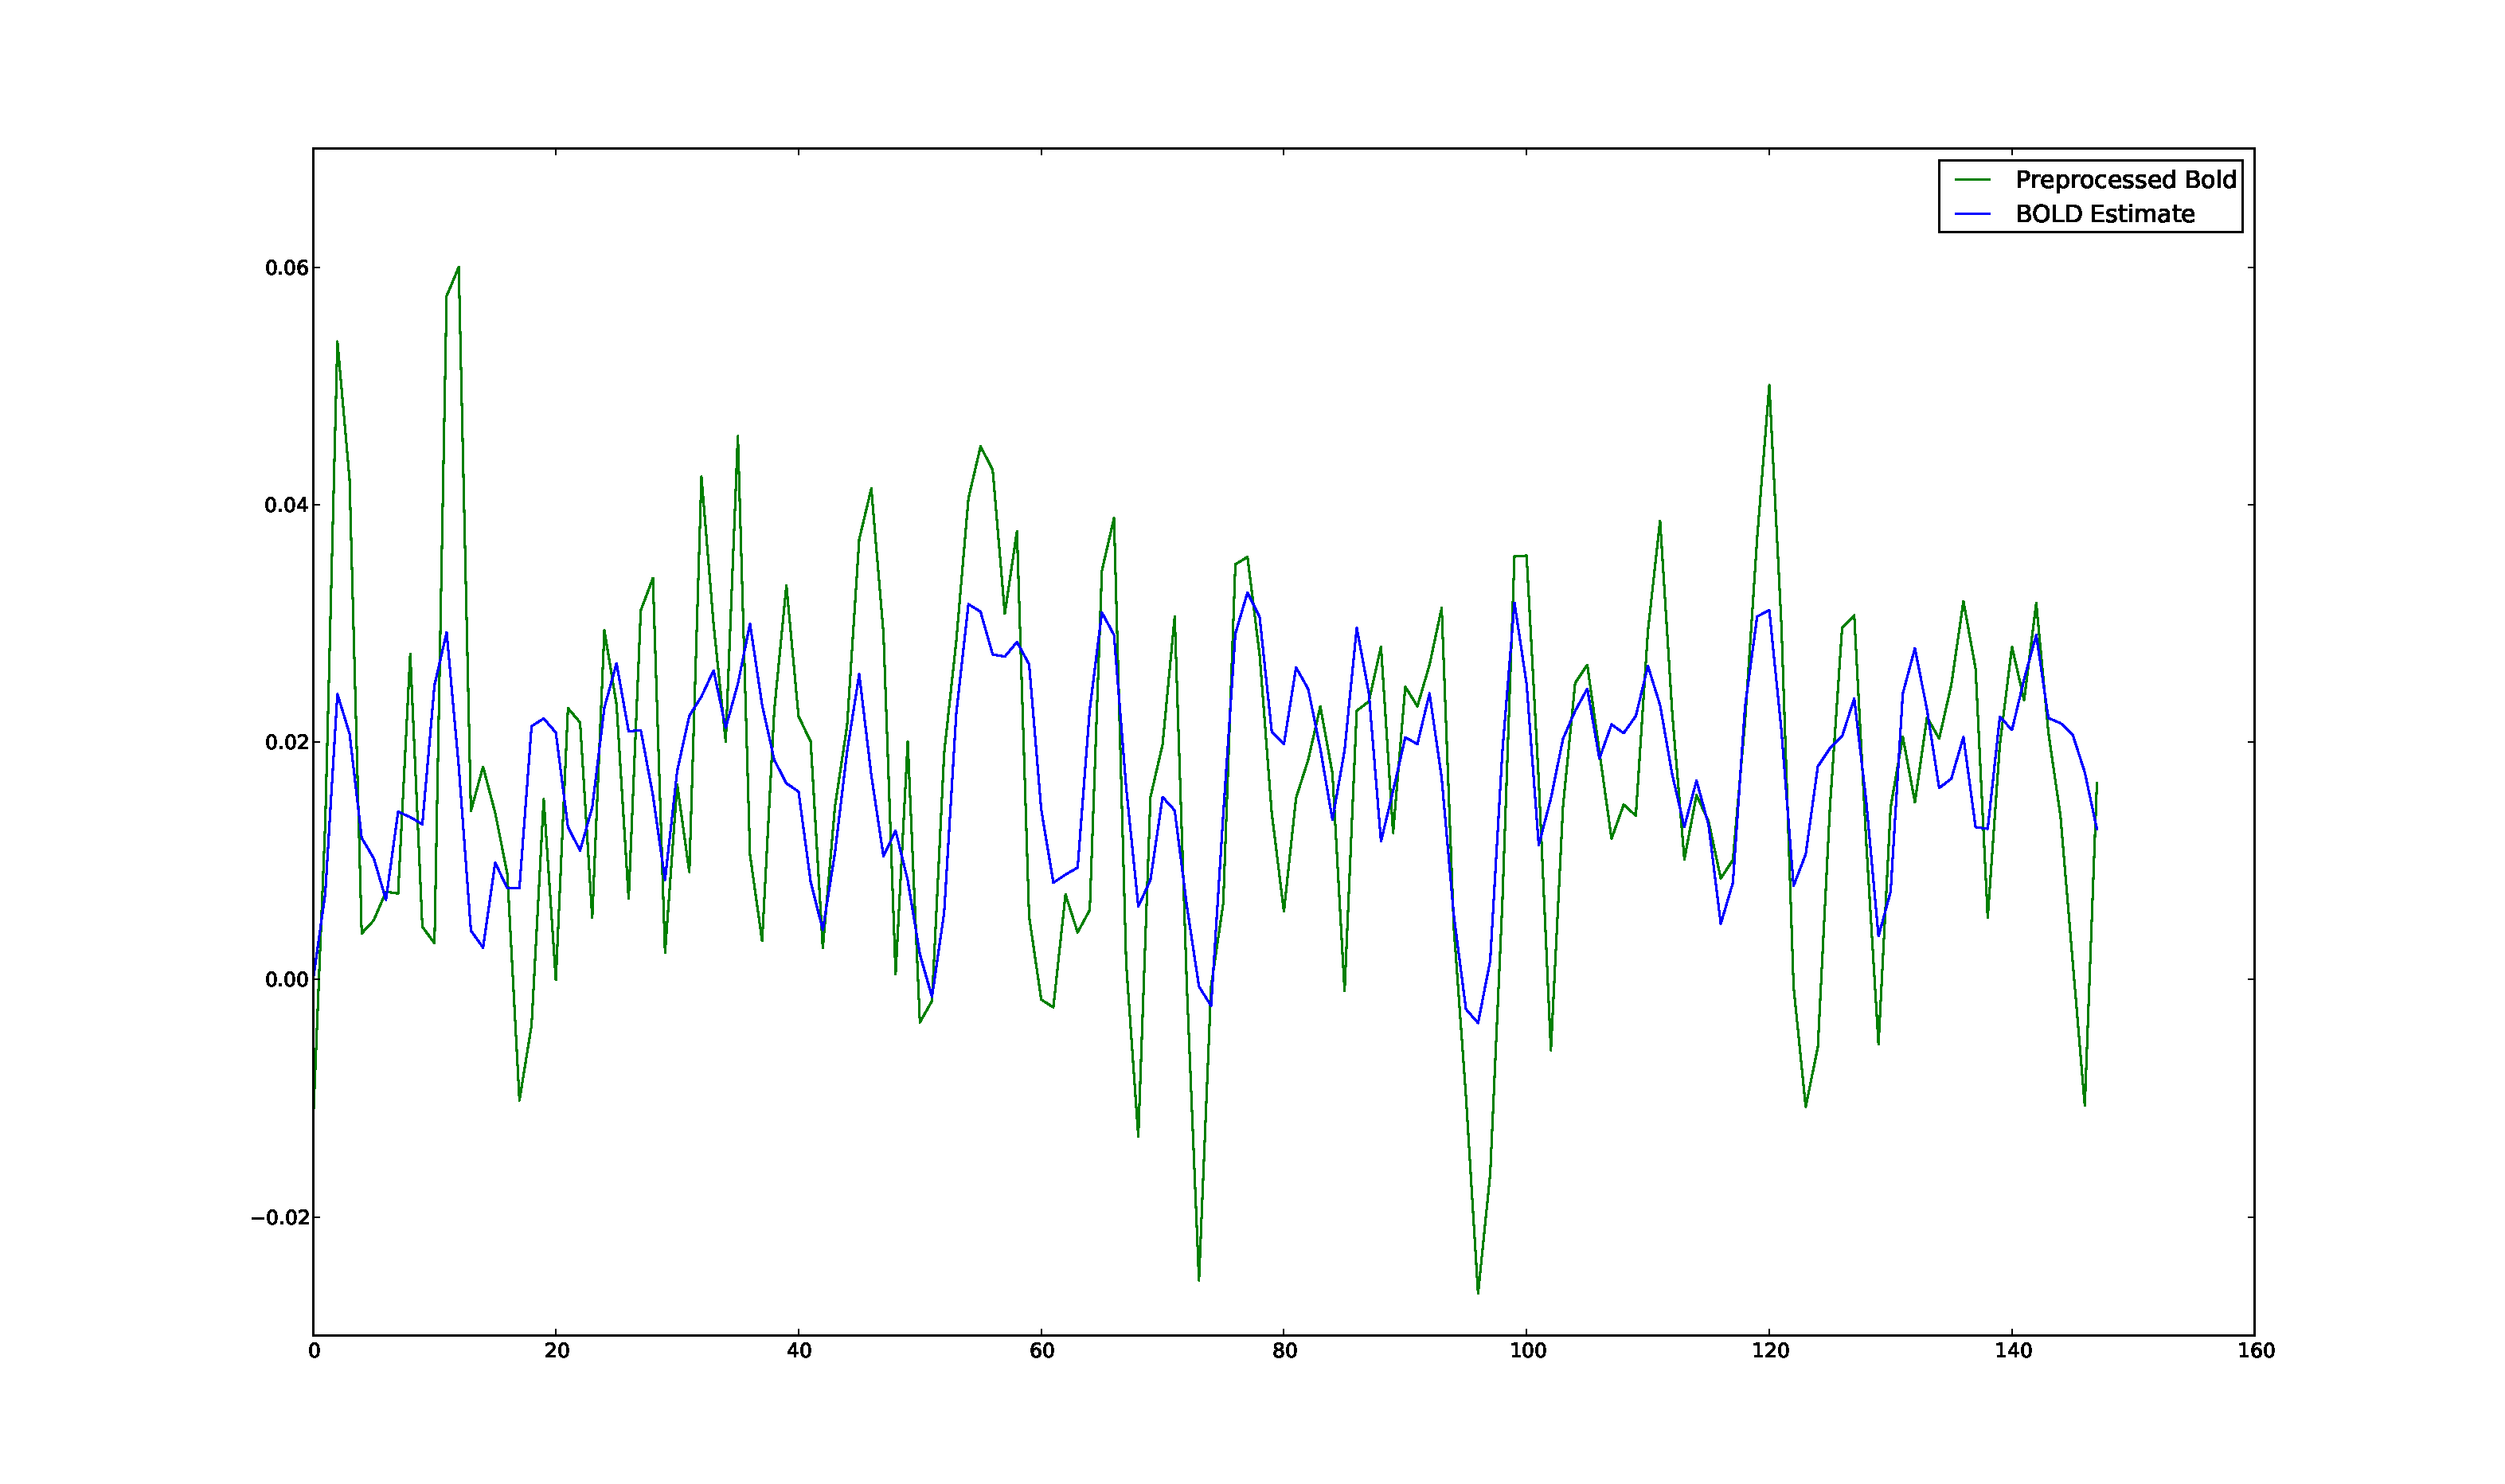
\includegraphics[clip=true,trim=5cm 1cm 4cm 1cm,width=15cm]{images/1_pfilter_37_14_7}}\\
\subfigure[SPM]{\label{fig:comp1spm} 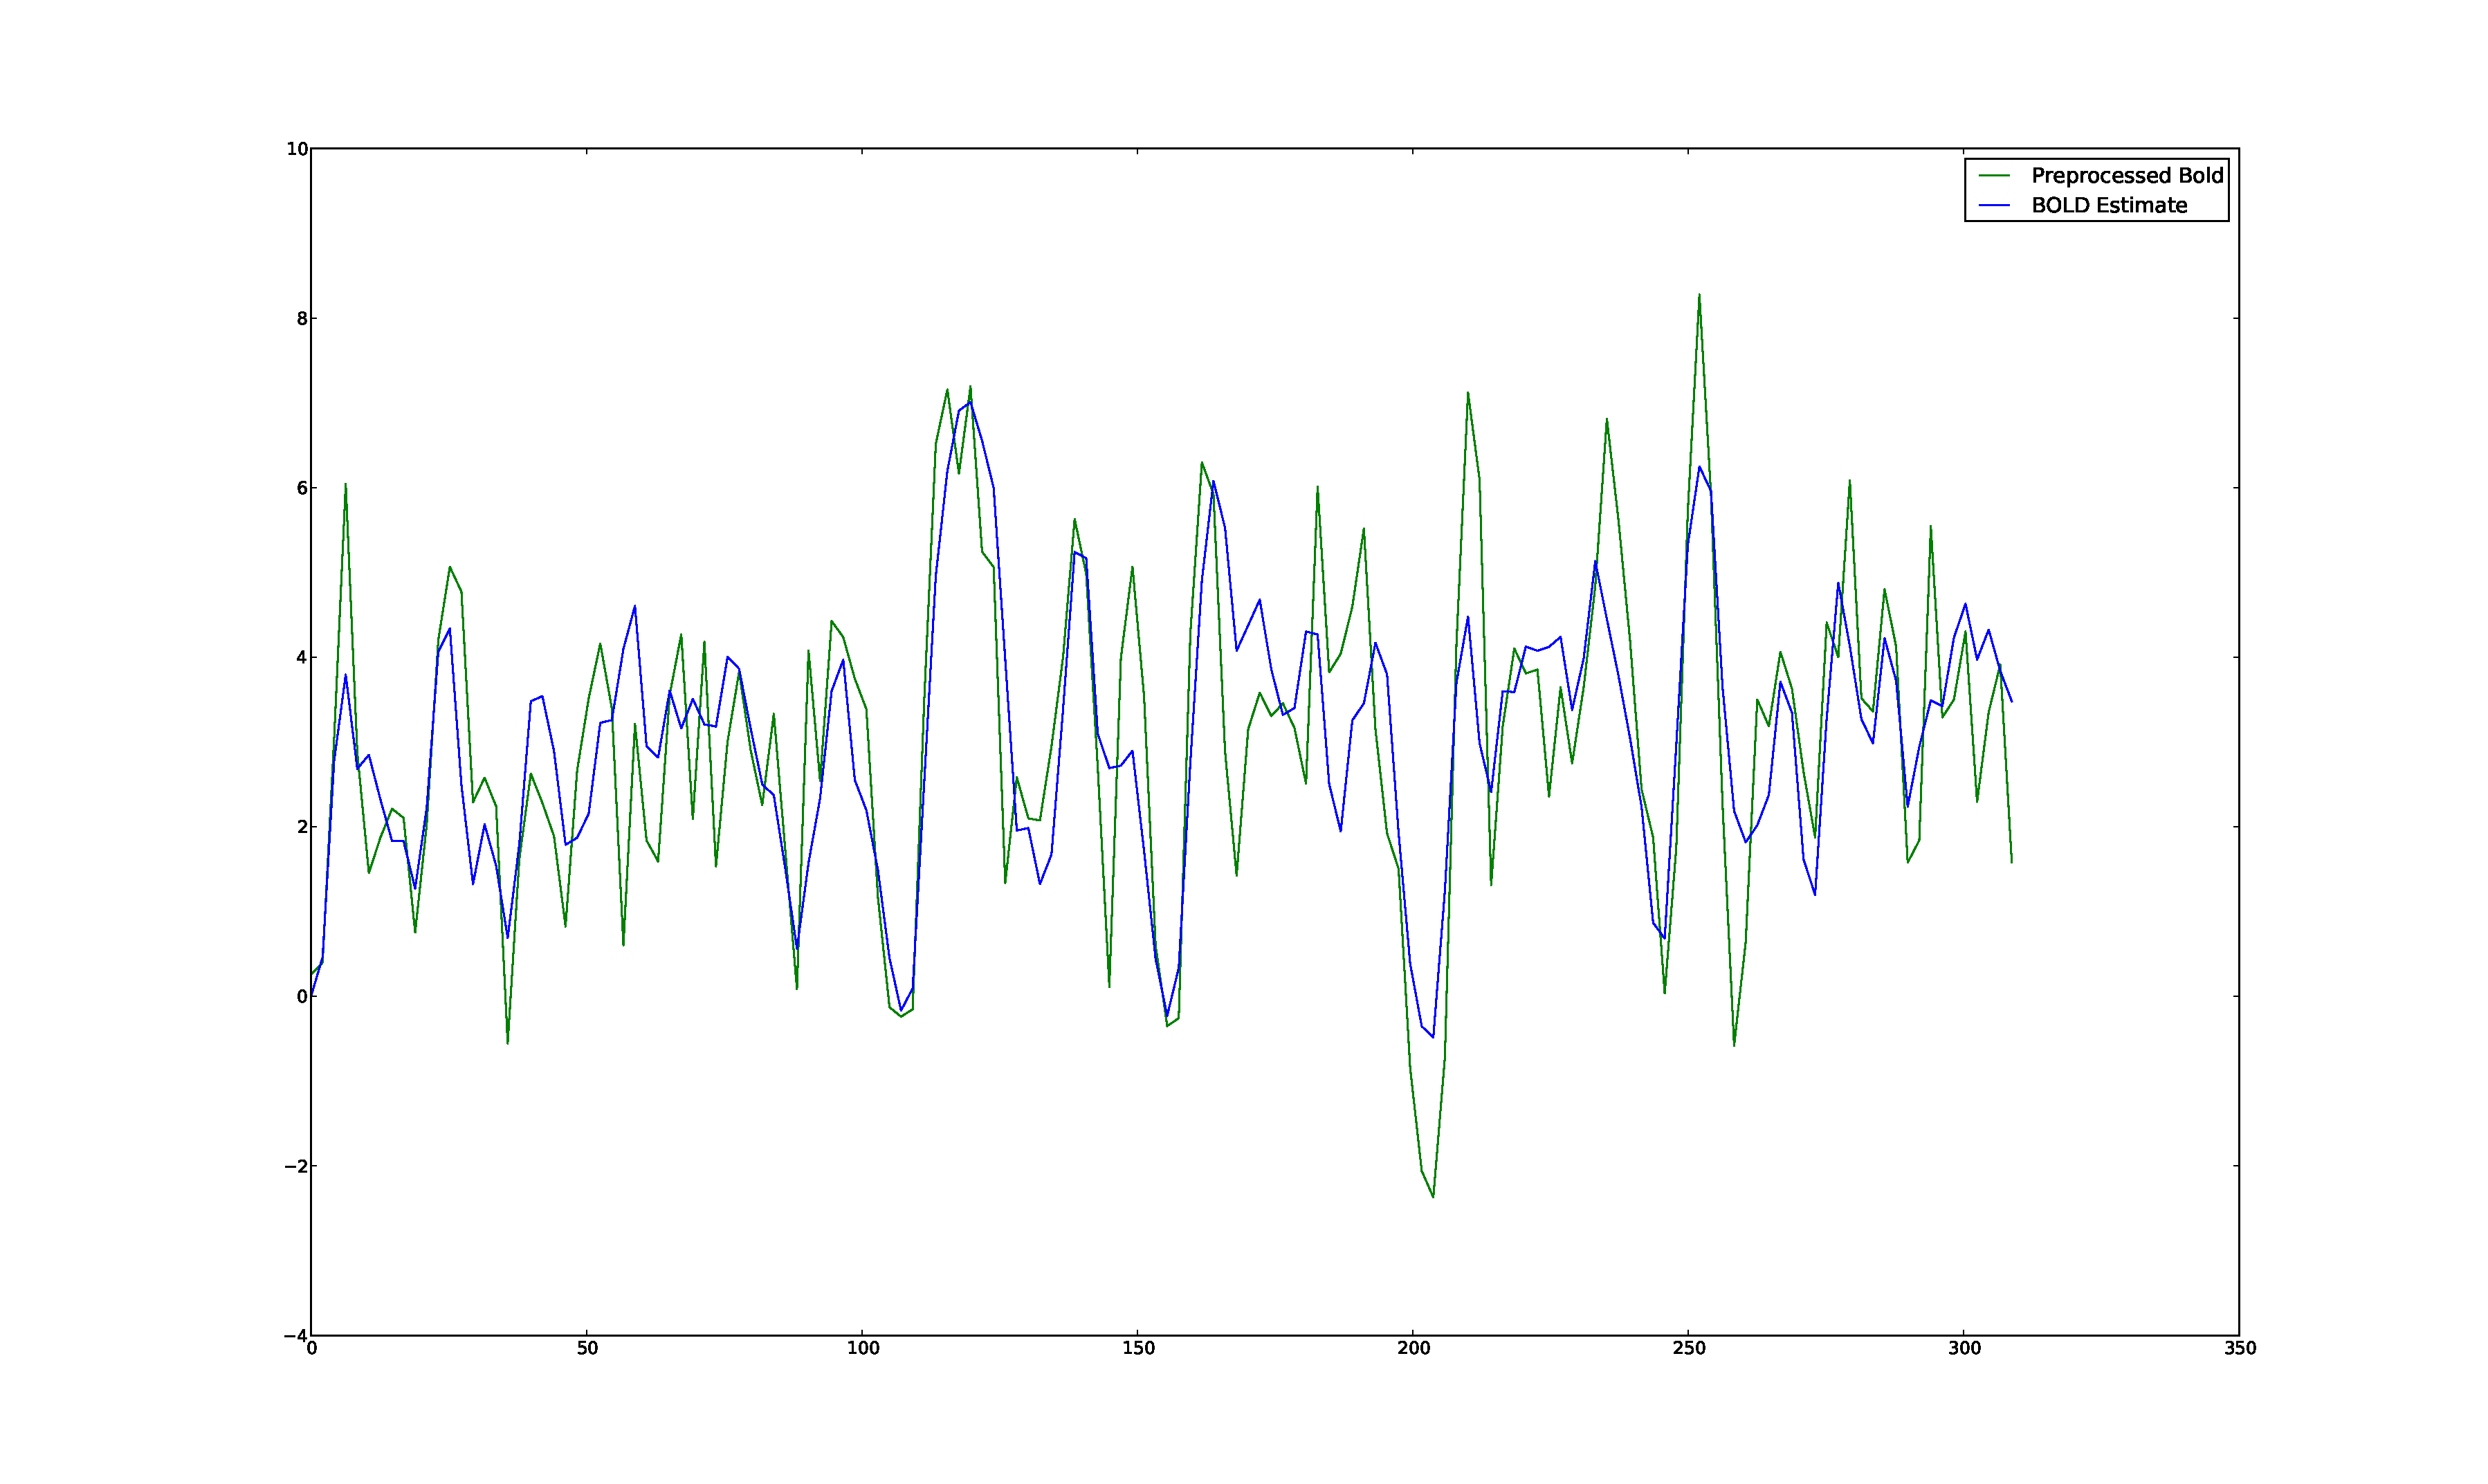
\includegraphics[clip=true,trim=5cm 1cm 4cm 1cm,width=15cm]{images/1_spm_37_14_7}}
\caption{Section 1, Estimated vs. Actual BOLD response. T-Score: $10.71$, Mutual Information: $0.33$, Residual: $0.72$.}
\label{fig:comp1}
\end{figure}

%34-12-7 
\begin{figure}
\subfigure[Particle Filter]{\label{fig:comp2pfilter} 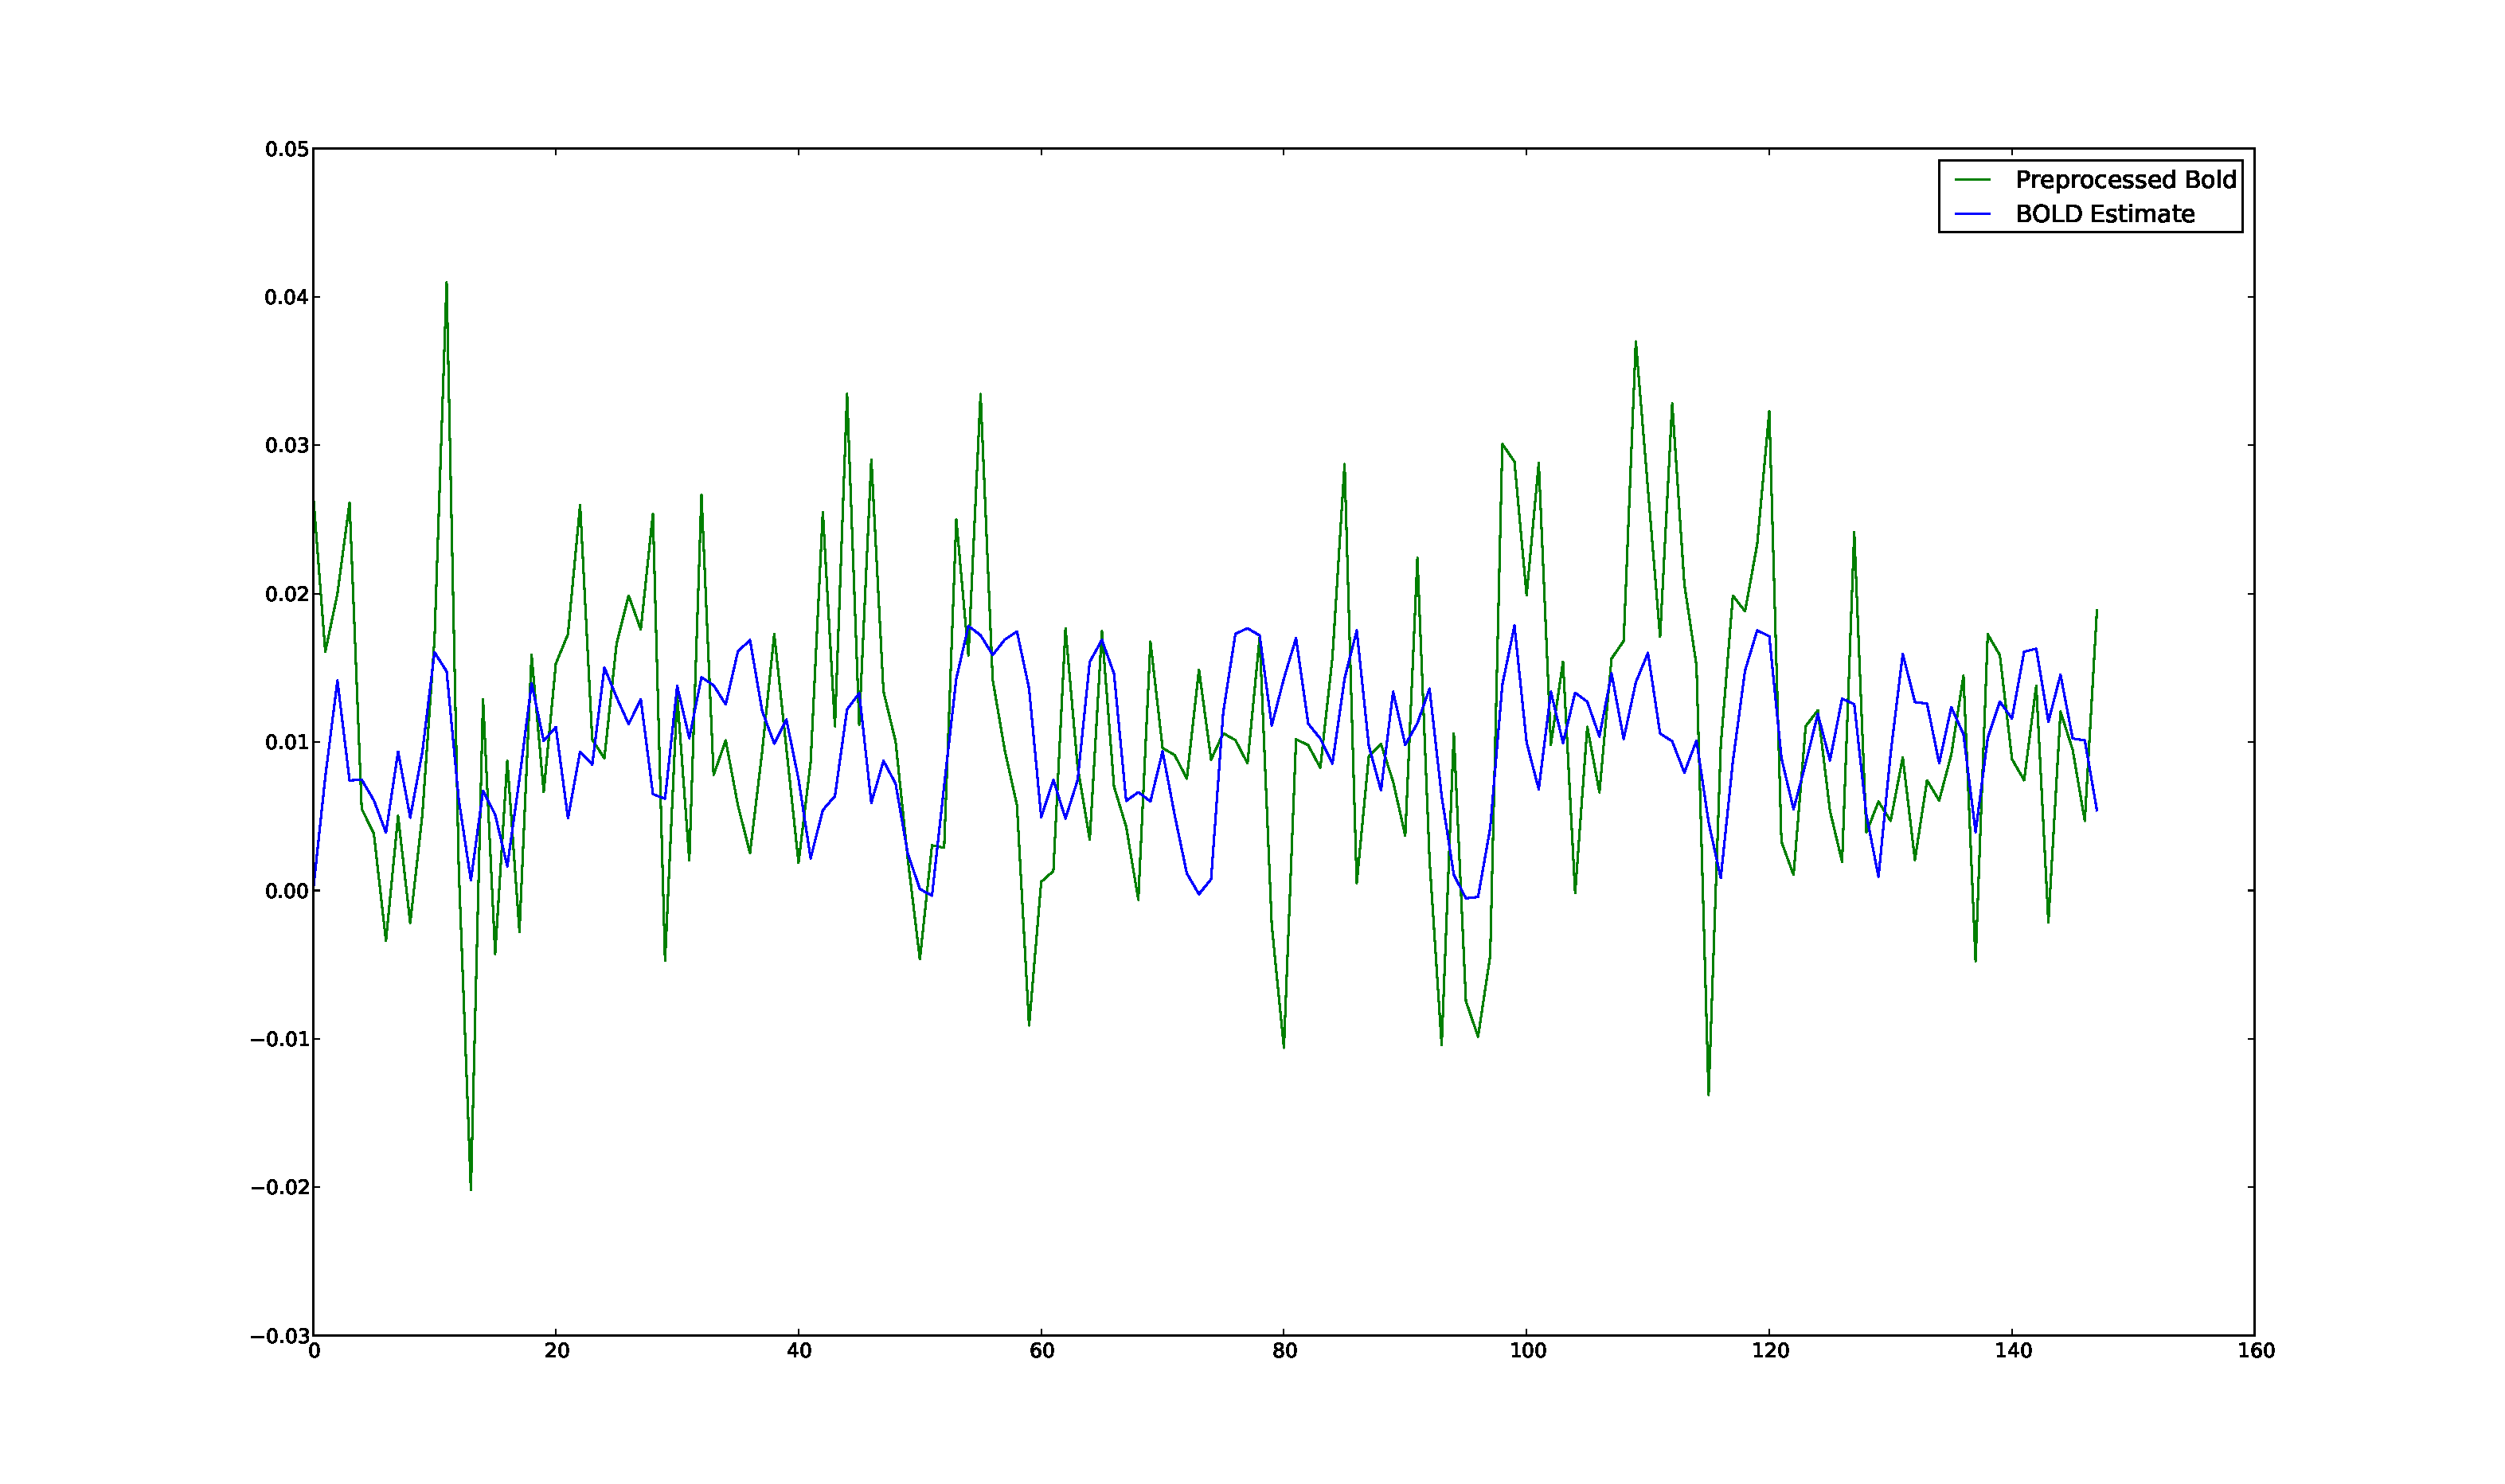
\includegraphics[clip=true,trim=5cm 1cm 4cm 1cm,width=15cm]{images/2_pfilter_34_12_7}}\\
\subfigure[SPM]{\label{fig:comp2spm} 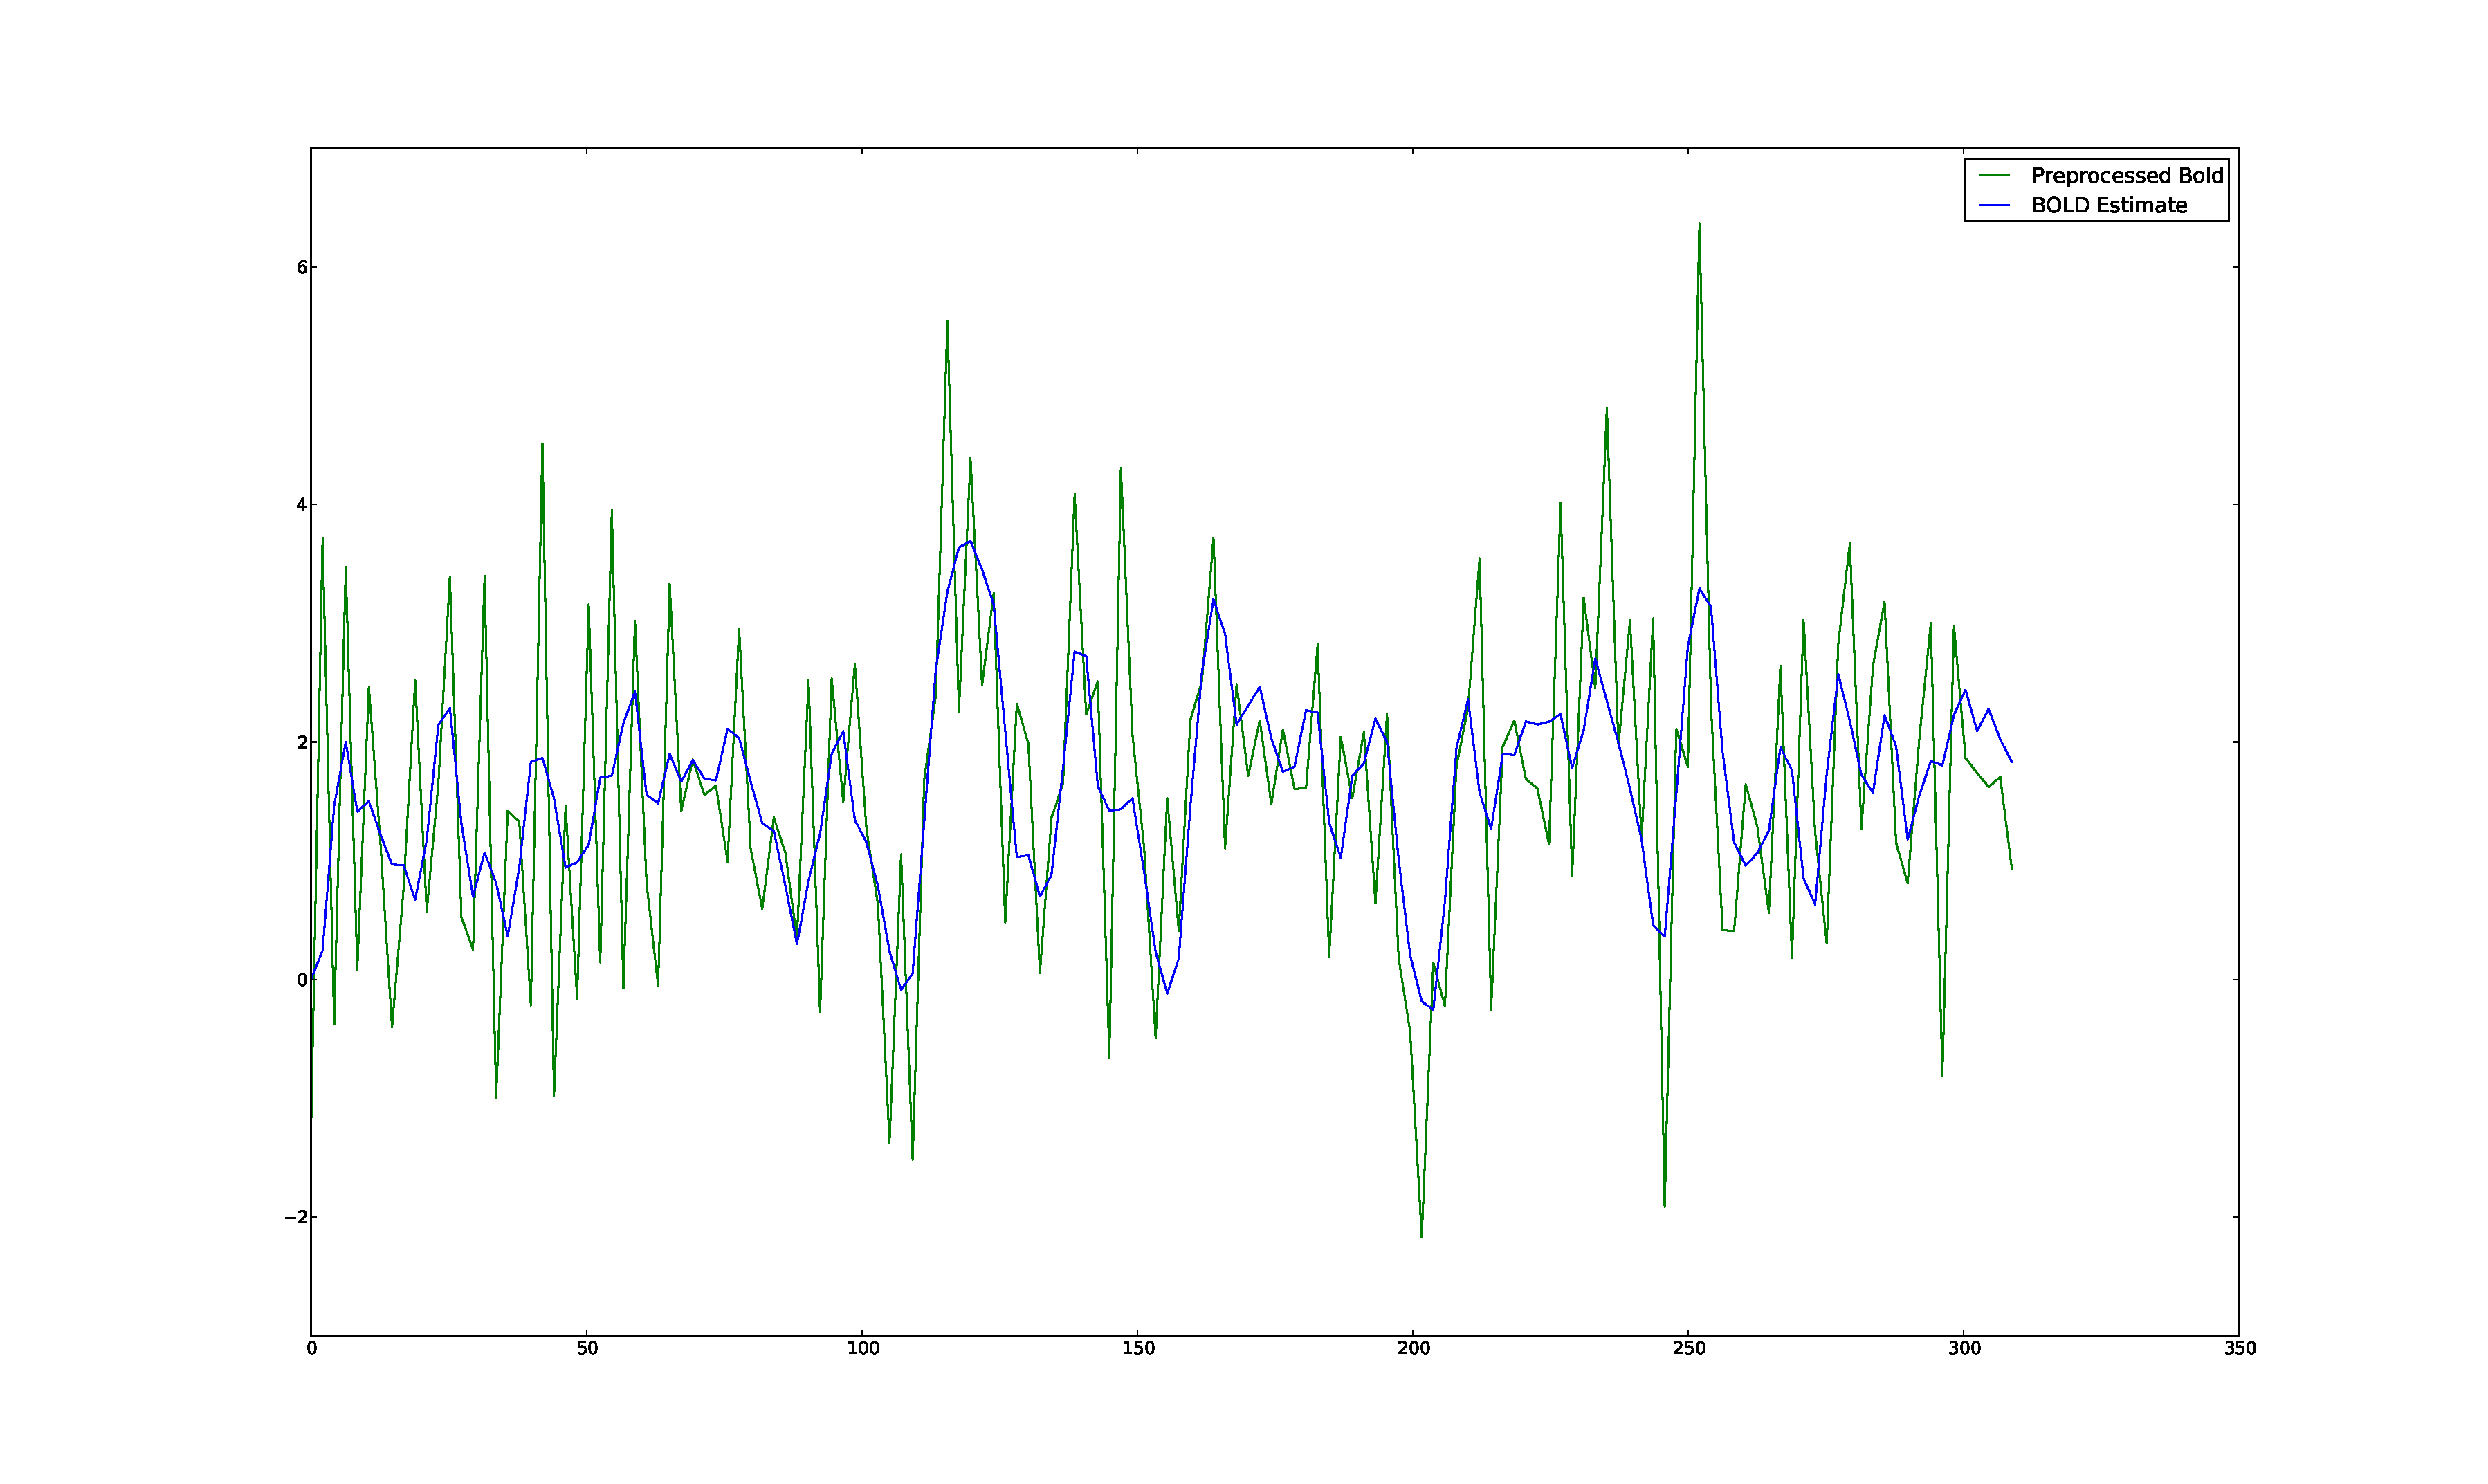
\includegraphics[clip=true,trim=5cm 1cm 4cm 1cm,width=15cm]{images/2_spm_34_12_7}}
\caption{Section 2, Estimated vs. Actual BOLD response. T-Score: $6.97$, Mutual Information: $0.04$, Residual: $1.02$.}
\label{fig:comp2}
\end{figure}

I chose several voxels to discuss further from \autoref{fig:hm_canon_pfilter} and \autoref{fig:hm_canon_spm}.
The first voxel, labeled 1, had a very high T-score, high mutual information,  as well as 
a low error (around $.7$). Thus, the
fit should be very good in both the SPM and particle filter output; this comparison is shown in 
\autoref{fig:comp1}. Recall that SPM worked on a slightly less noisy time series because of the
spatial smoothing; this explains the lack of the sharp peak in the particle filter's preprocessed
data. Regardless, as expected, both work. 

I chose the second voxel (\autoref{fig:comp2}) because it was active in SPM and it would appear to be in a prime
location to be active in the SPM image (given the results in the surrounding voxels). The fit,
however shows just why the residual was high and the mutual information was low. This is a
prime example of a false positive due to the large smoothing kernel applied by SPM. 
For instance at 75 seconds, the stimulus is not present, and so the signal should drop off; yet
it doesn't. While a few peaks seem to match, most of the signal does not correlate with the
expected state progression. This voxel is not being driven direcly by the input, although it
may be gated or driven through intermediate region. 

The third voxel, compared in \autoref{fig:comp3}, was far away from any other active voxels 
and yet had a very low (around $.7$) residual. At the same time, the mutual information was
high enough to make the point suspect. Although the estimated signal seems to run down the
middle of the measurement signal; it is clear that there is a significant amount of noise
present in the signal that is not being explained by the particle filter, 
In both preprocessed time-series the input is extremely noisy, yet by the normalized residual 
the response is good. This is an example of a false positive from the residual metric. 

The fourth voxel (\autoref{fig:comp4}) selected for anyalysis had a relatively high residual, and was not picked
for activation by SPM. The mutual information was only $0.06$
for the image. It is simple to see why the residual was not acceptable in this case.
At the same time, the peaks do seem to correlate with the measurement peaks. Regardless,
this is an example of a  false positive from the mutual information metric. 

The fifth voxel (\autoref{fig:comp5}) is an example of a region with increased activation
due to smoothing. The fit provided by the BOLD particle filter is not very good, and the time
series input to SPM is far less noisy. Regardless this is another case where the peaks
seem to match, yet nothing else does. Take for instance the measurements from $30$ seconds
to $40$ seconds. At that point there is a significant spike in the BOLD signal, yet the
actual measured signal declines. This is an indication that the BOLD signal is not directly
being driven by the input. It is likeley that the cause of the activation in this reason is
not true activation, but recieved from surrounding active regions through spatial smoothing. 

%23-21-7
\begin{figure}
\subfigure[Particle Filter]{\label{fig:comp3pfilter} 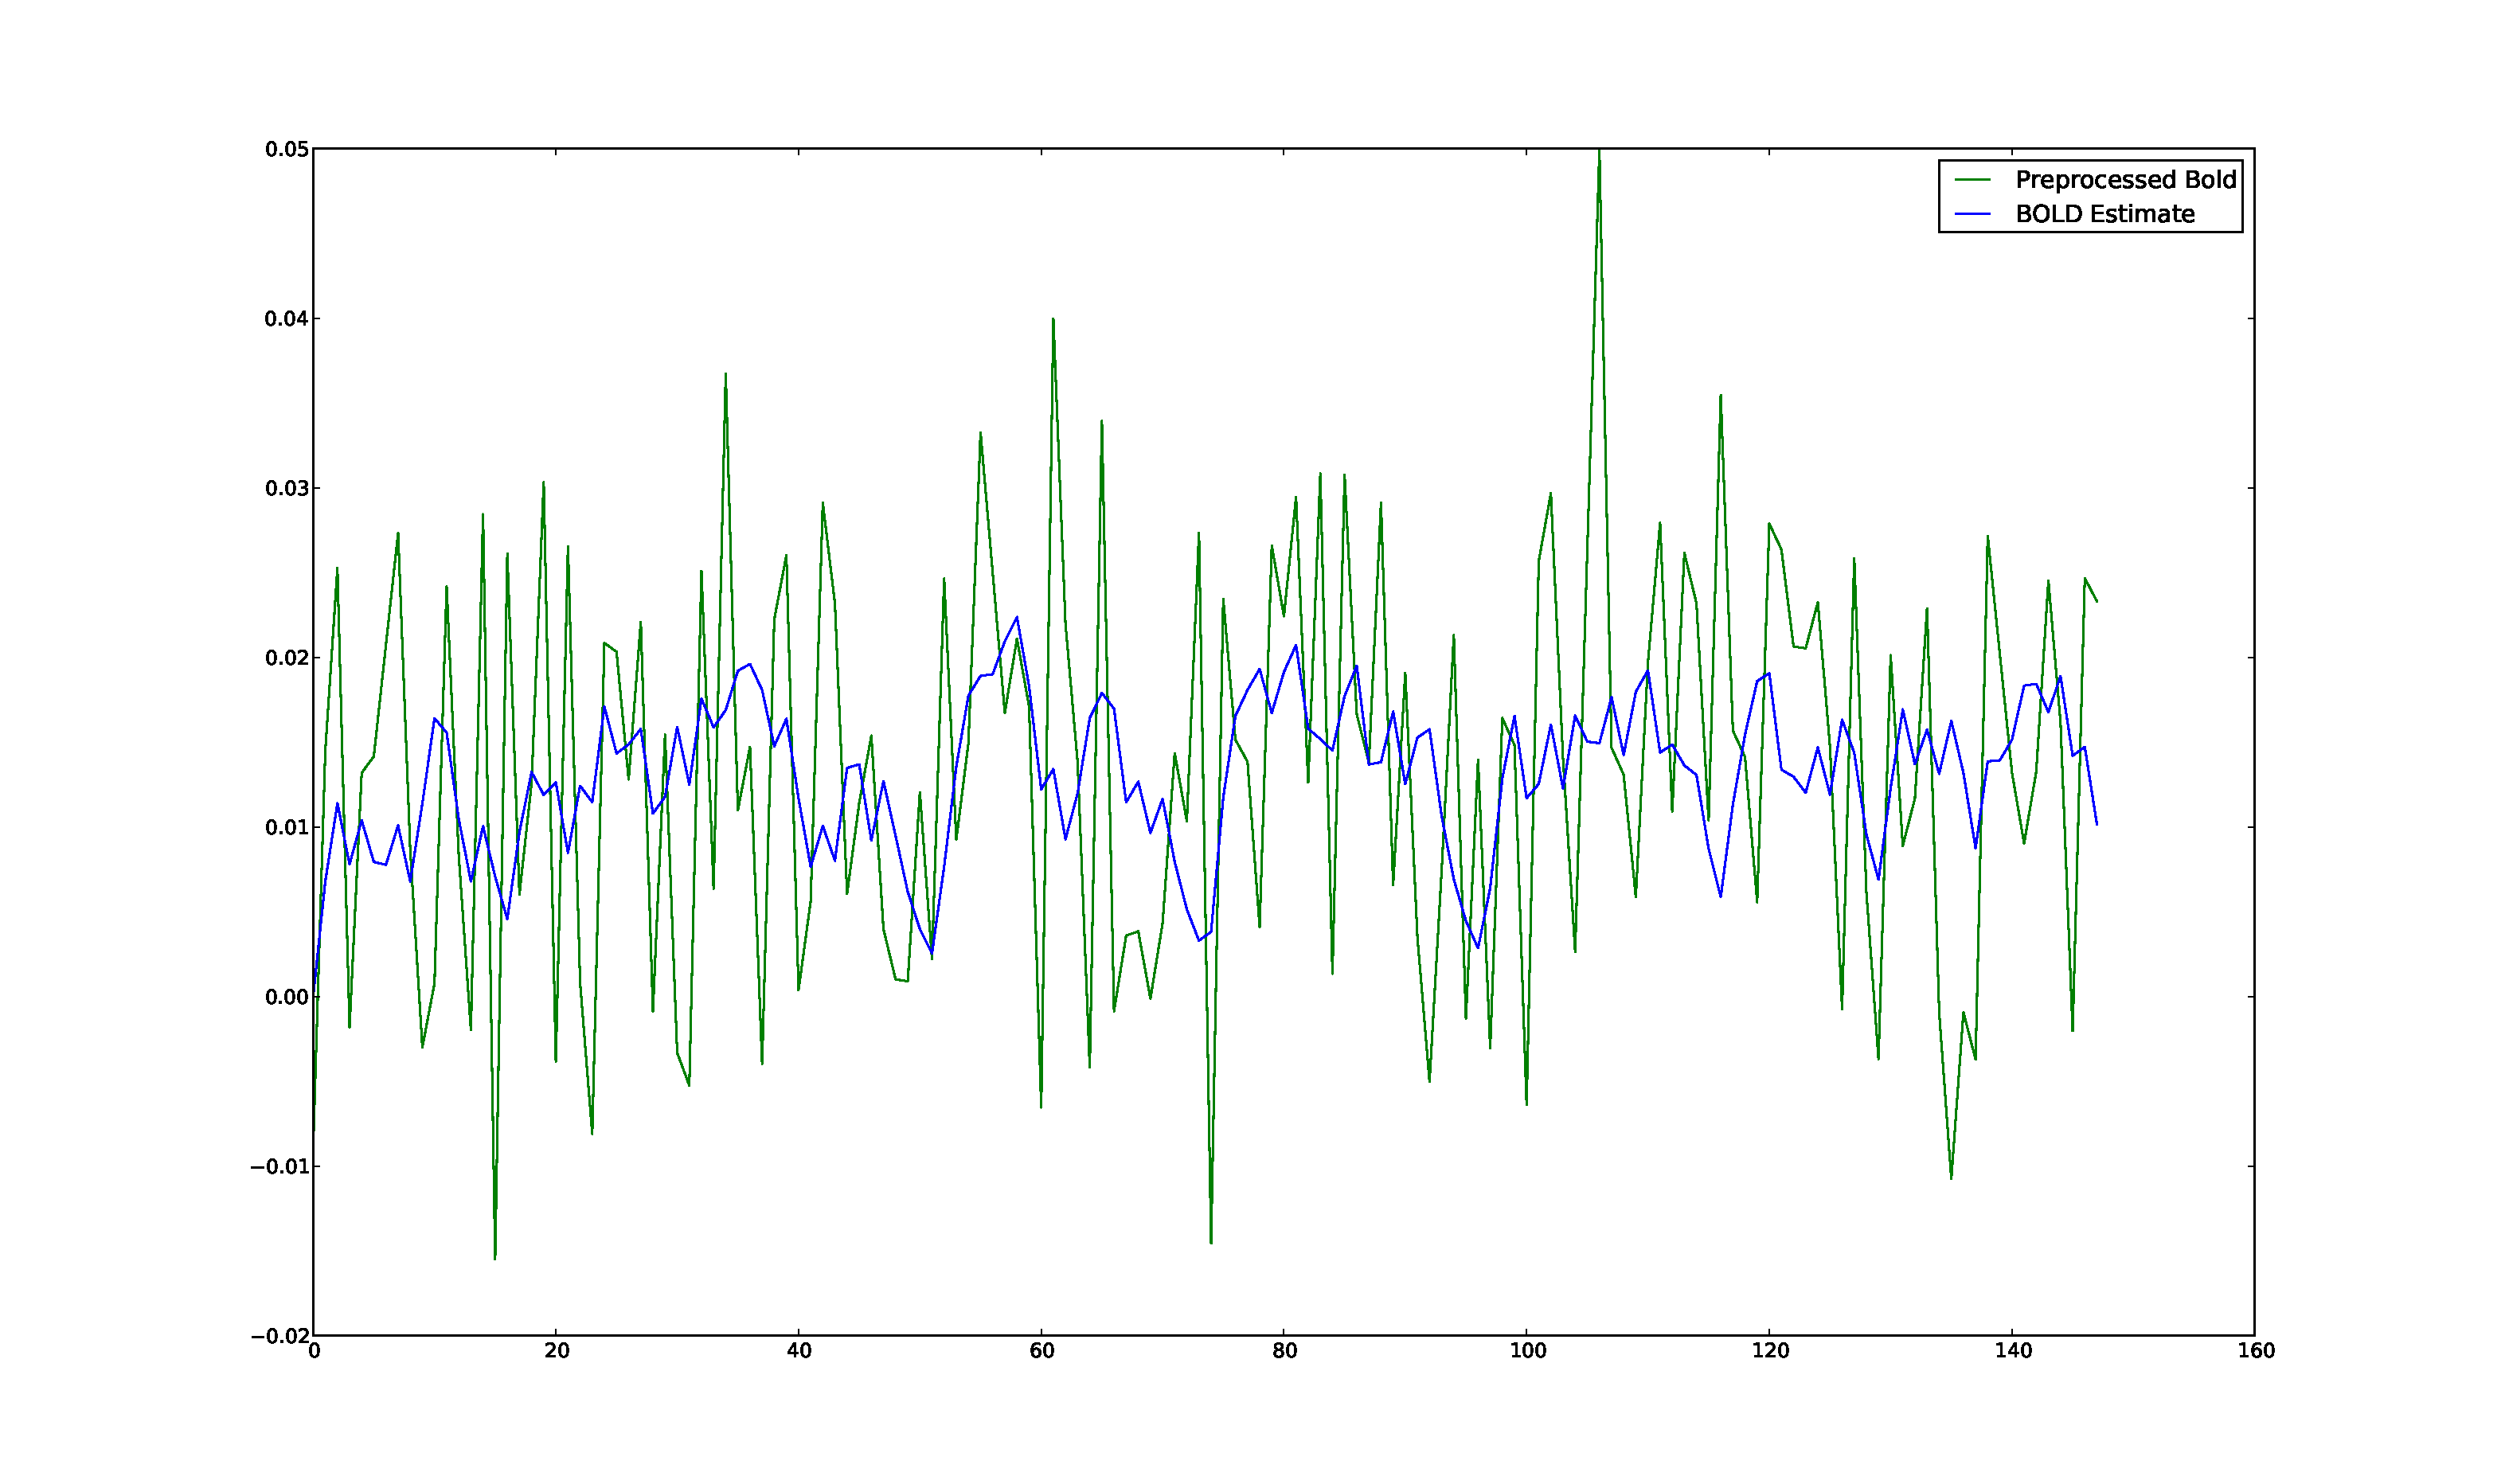
\includegraphics[clip=true,trim=5cm 1cm 4cm 1cm,width=15cm]{images/3_pfilter_23_21_7}}\\
\subfigure[SPM]{\label{fig:comp3spm} 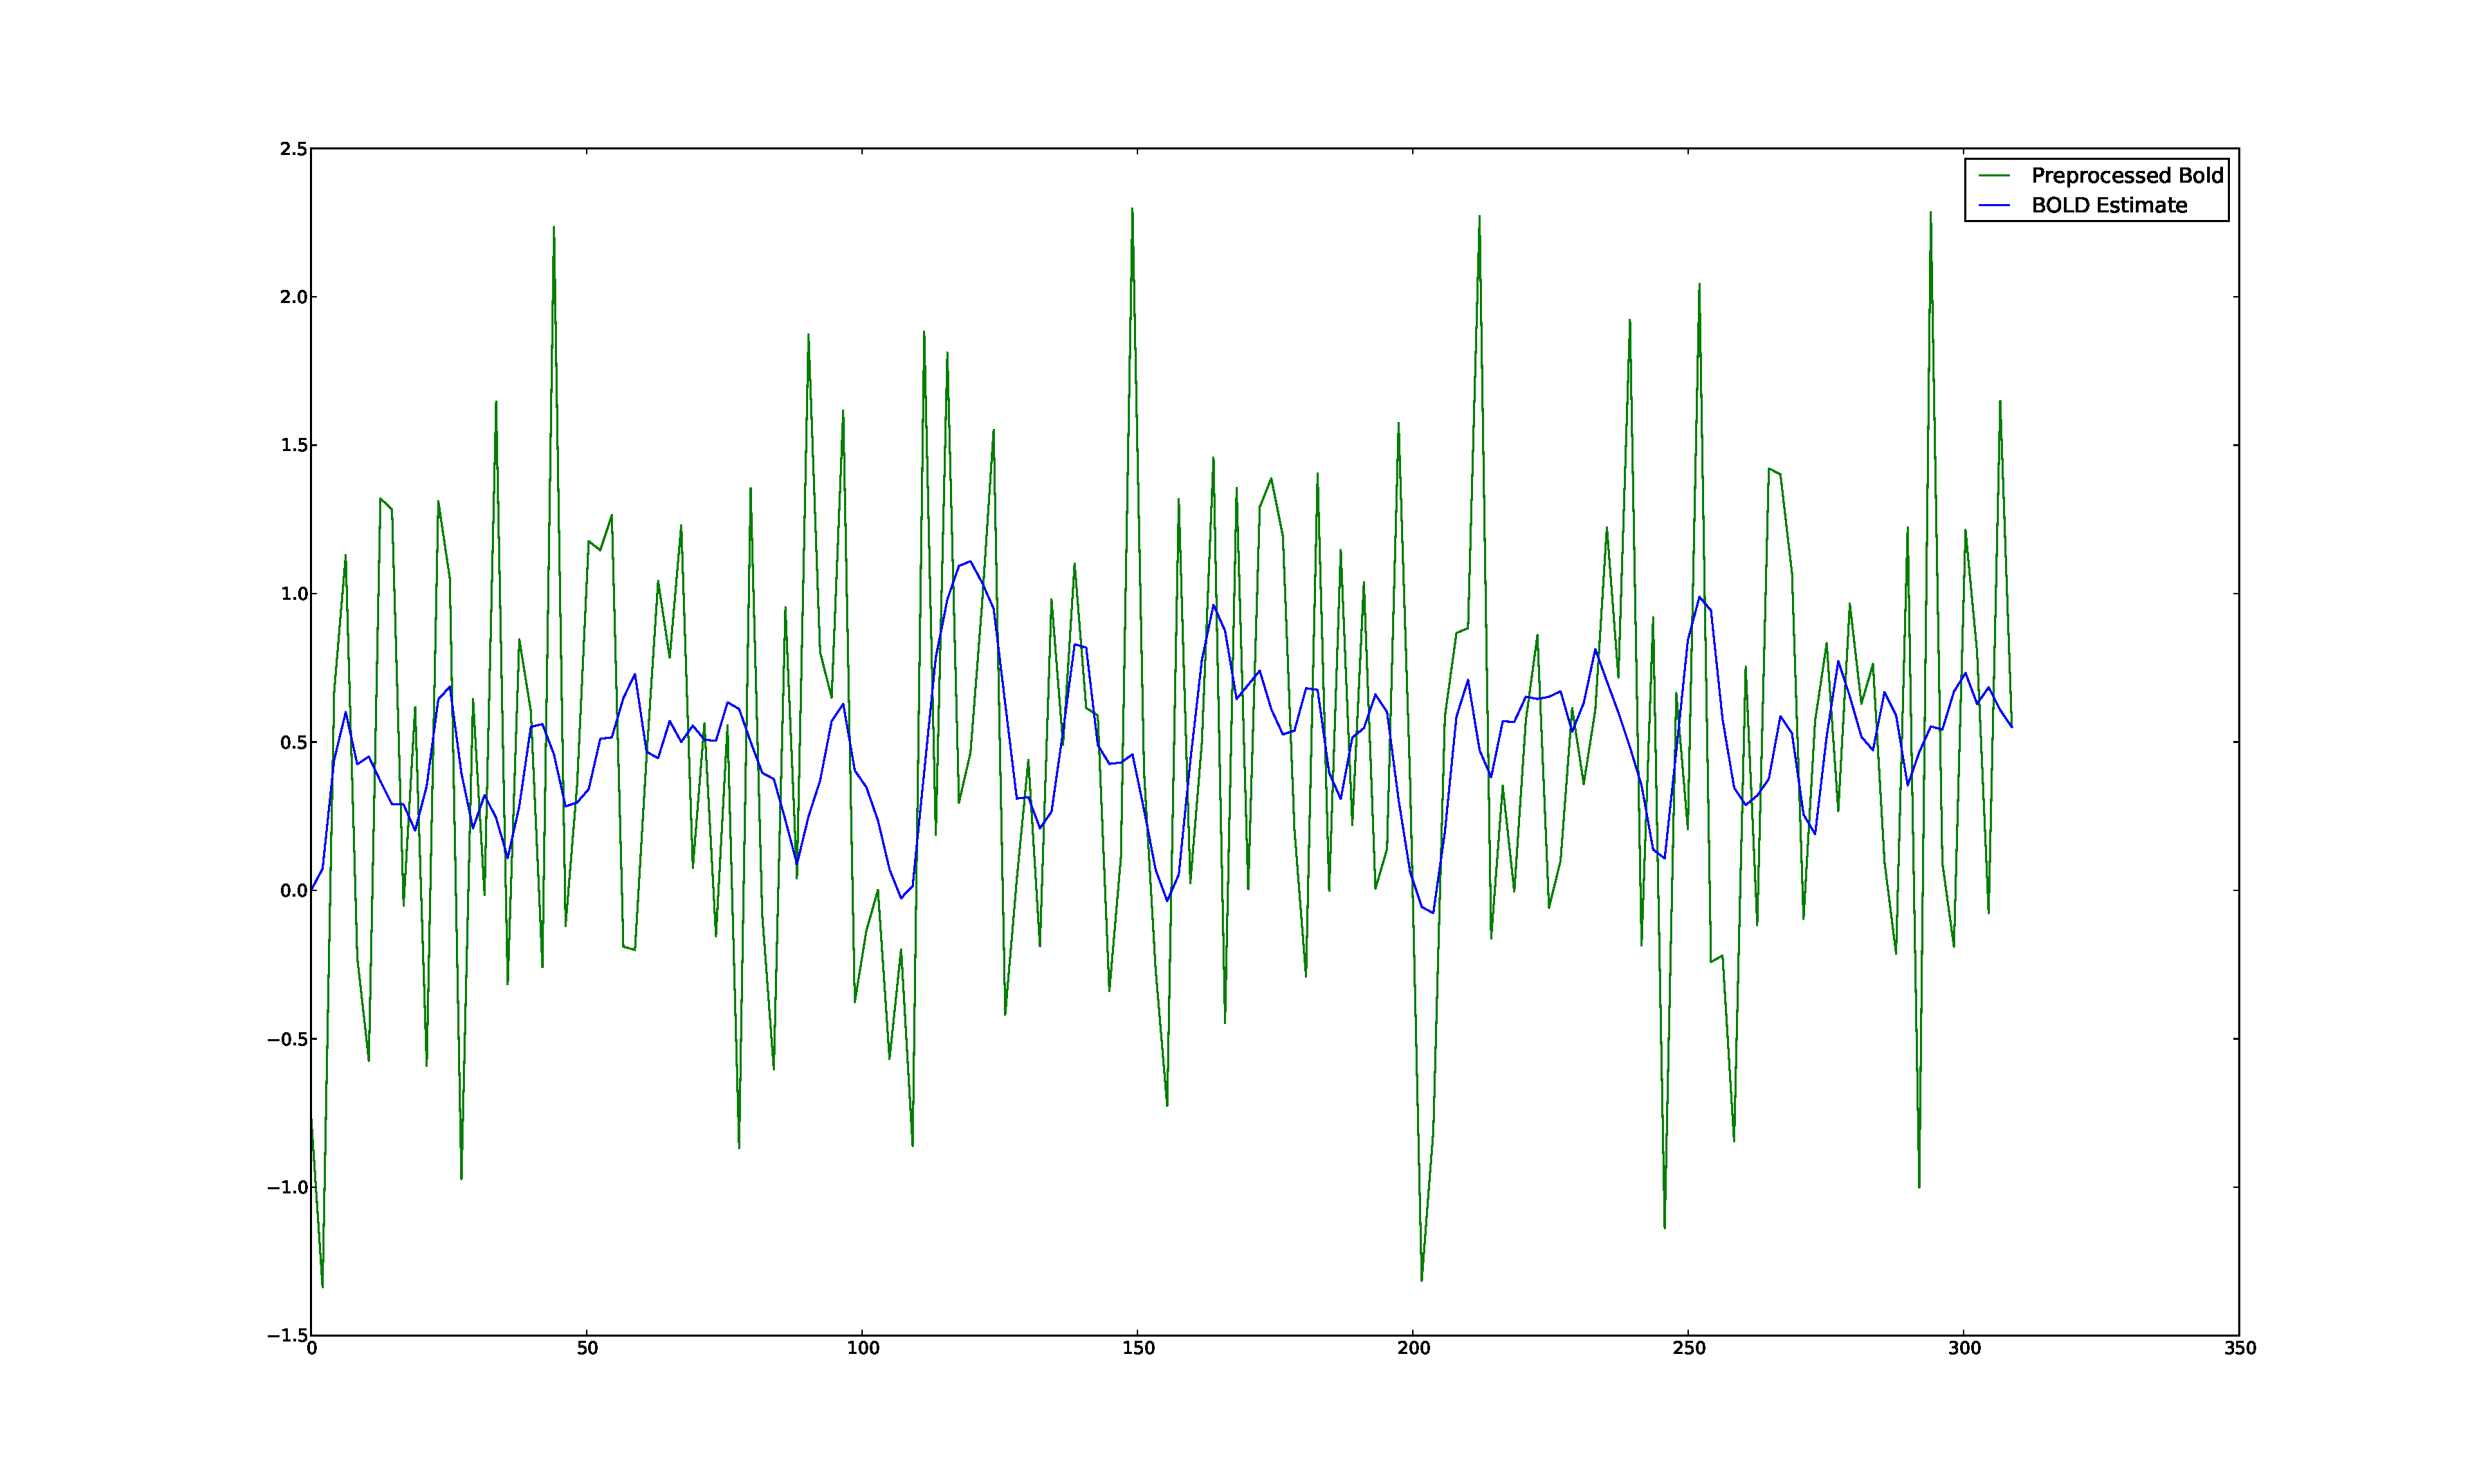
\includegraphics[clip=true,trim=5cm 1cm 4cm 1cm,width=15cm]{images/3_spm_23_21_7}}
\caption{Section 3, Estimated vs. Actual BOLD response. T-Score: $2.85$, Mutual Information: $-0.03$, Residual: $0.81$.}
\label{fig:comp3}
\end{figure}

%33-30-4
\begin{figure}[H]
\subfigure[Particle Filter]{\label{fig:comp4pfilter} 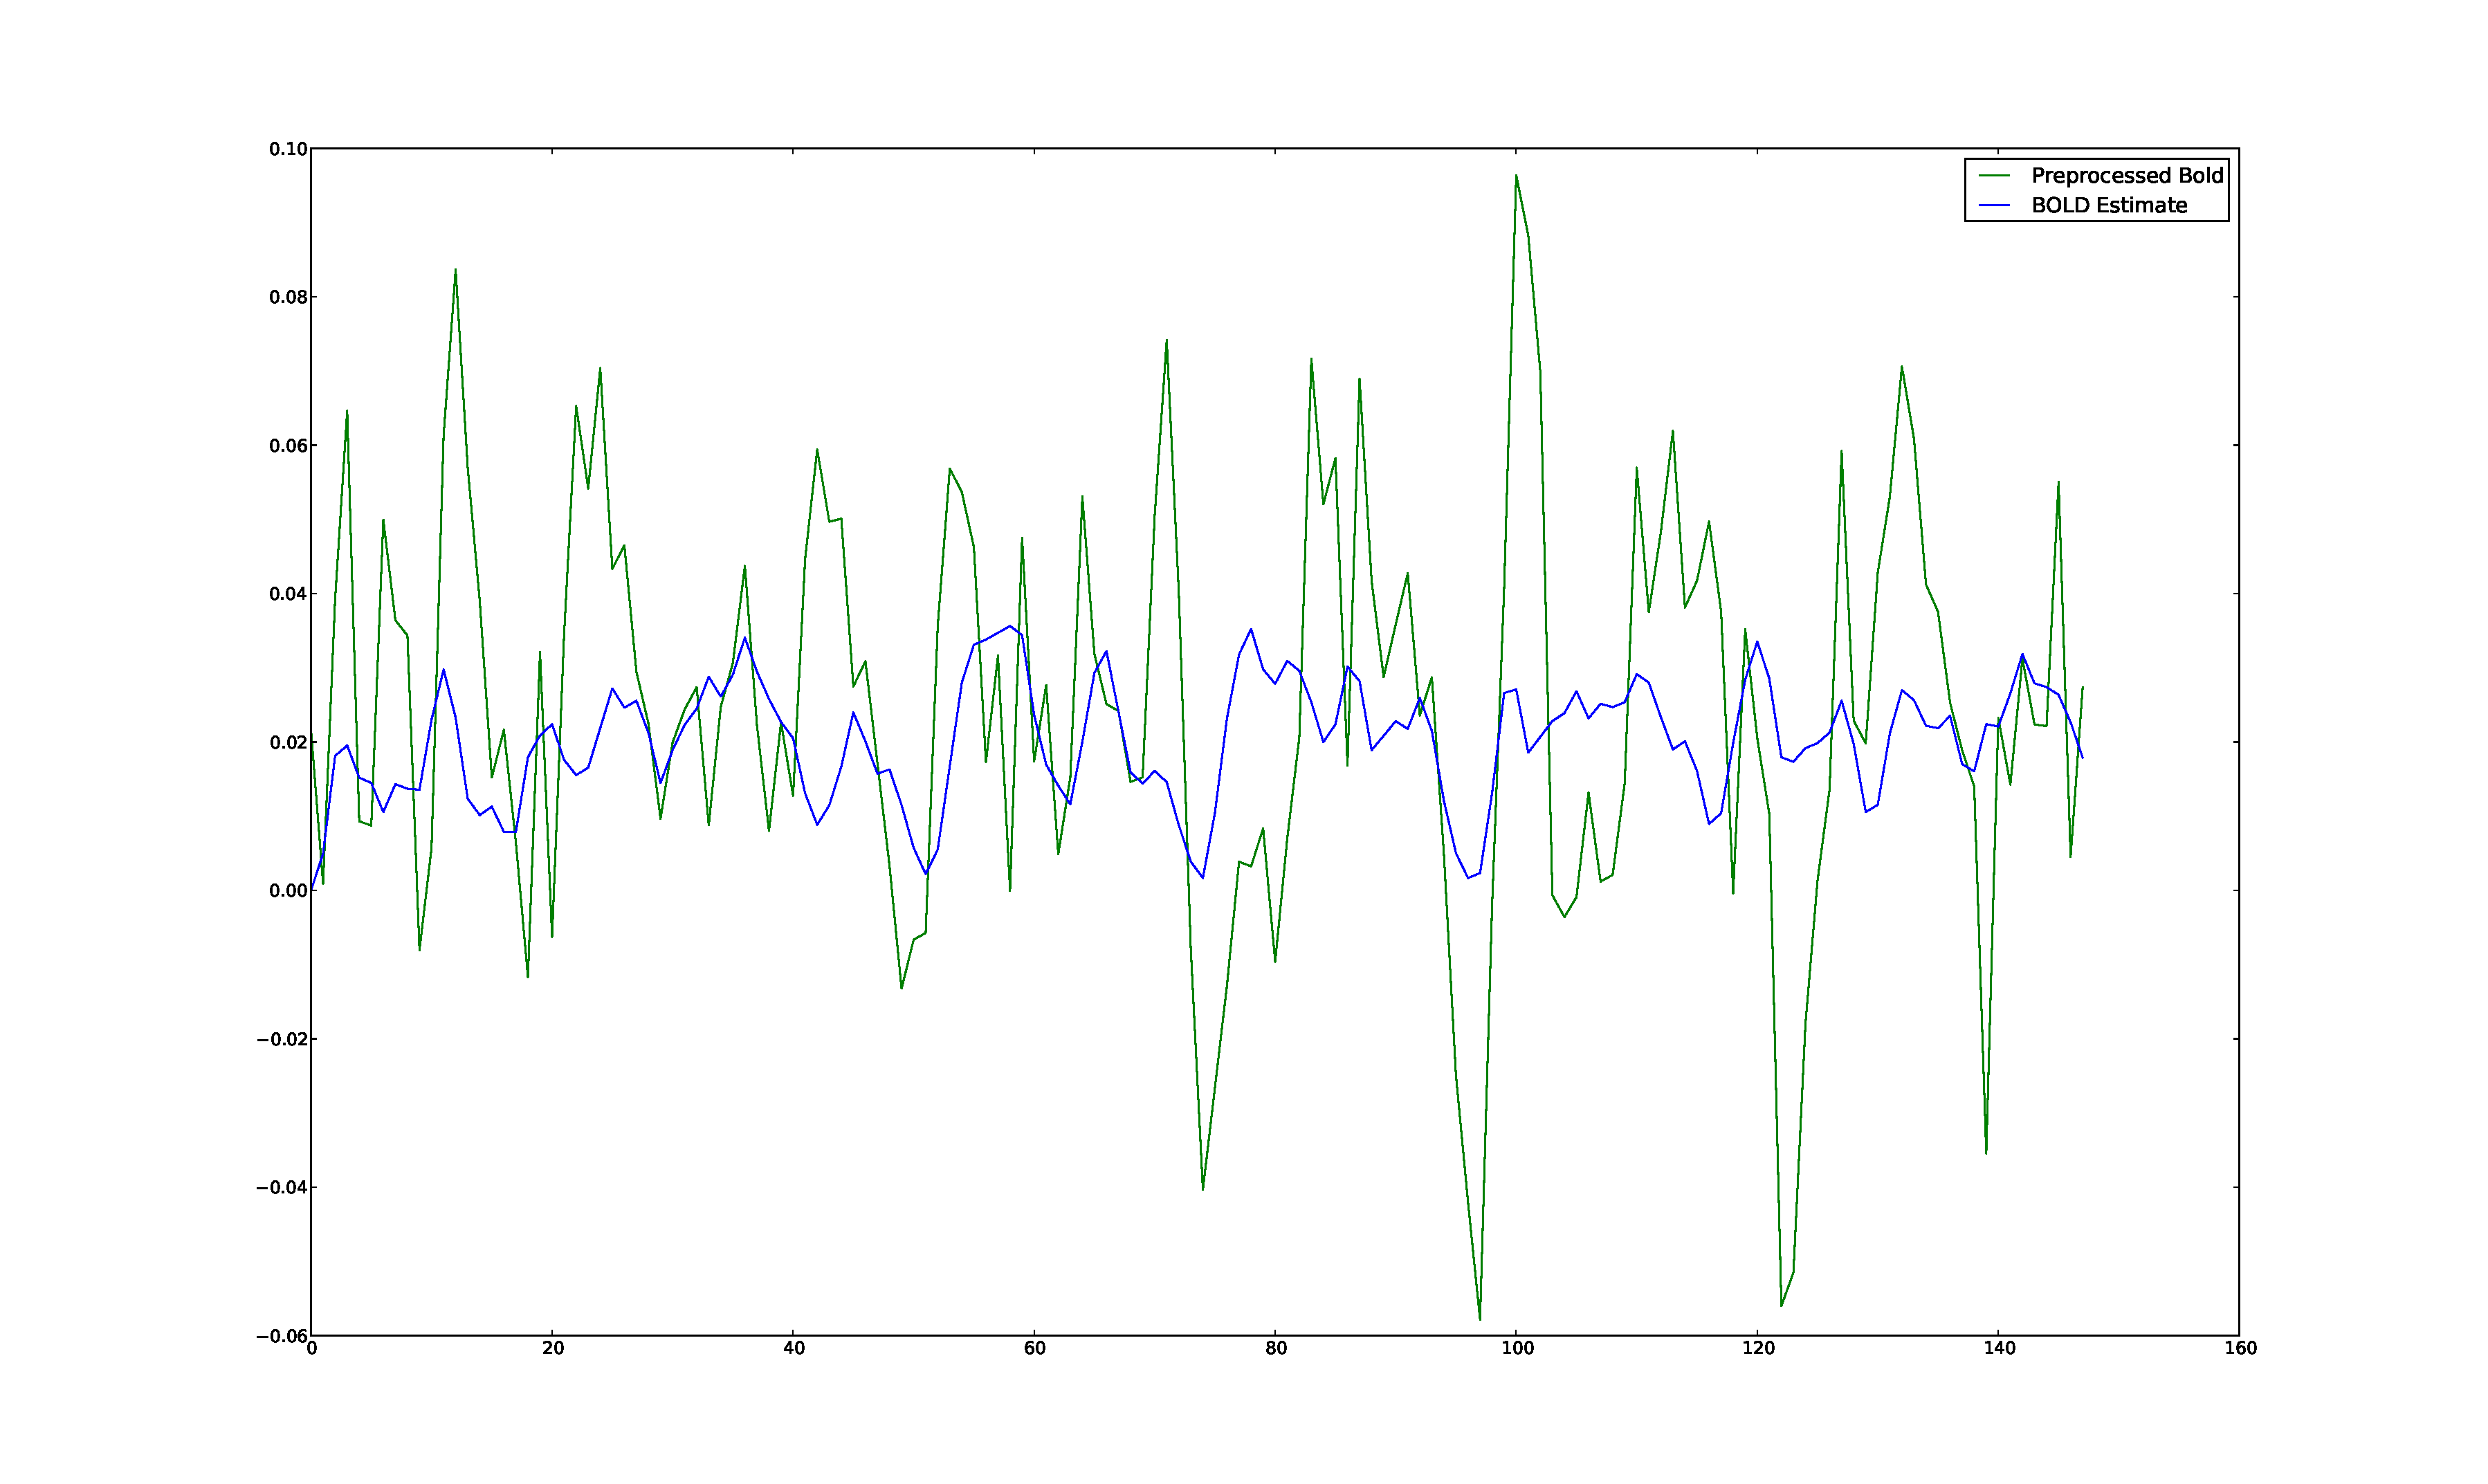
\includegraphics[clip=true,trim=5cm 1cm 4cm 1cm,width=15cm]{images/4_pfilter_26_15_7}}\\
\subfigure[SPM]{\label{fig:comp4spm} 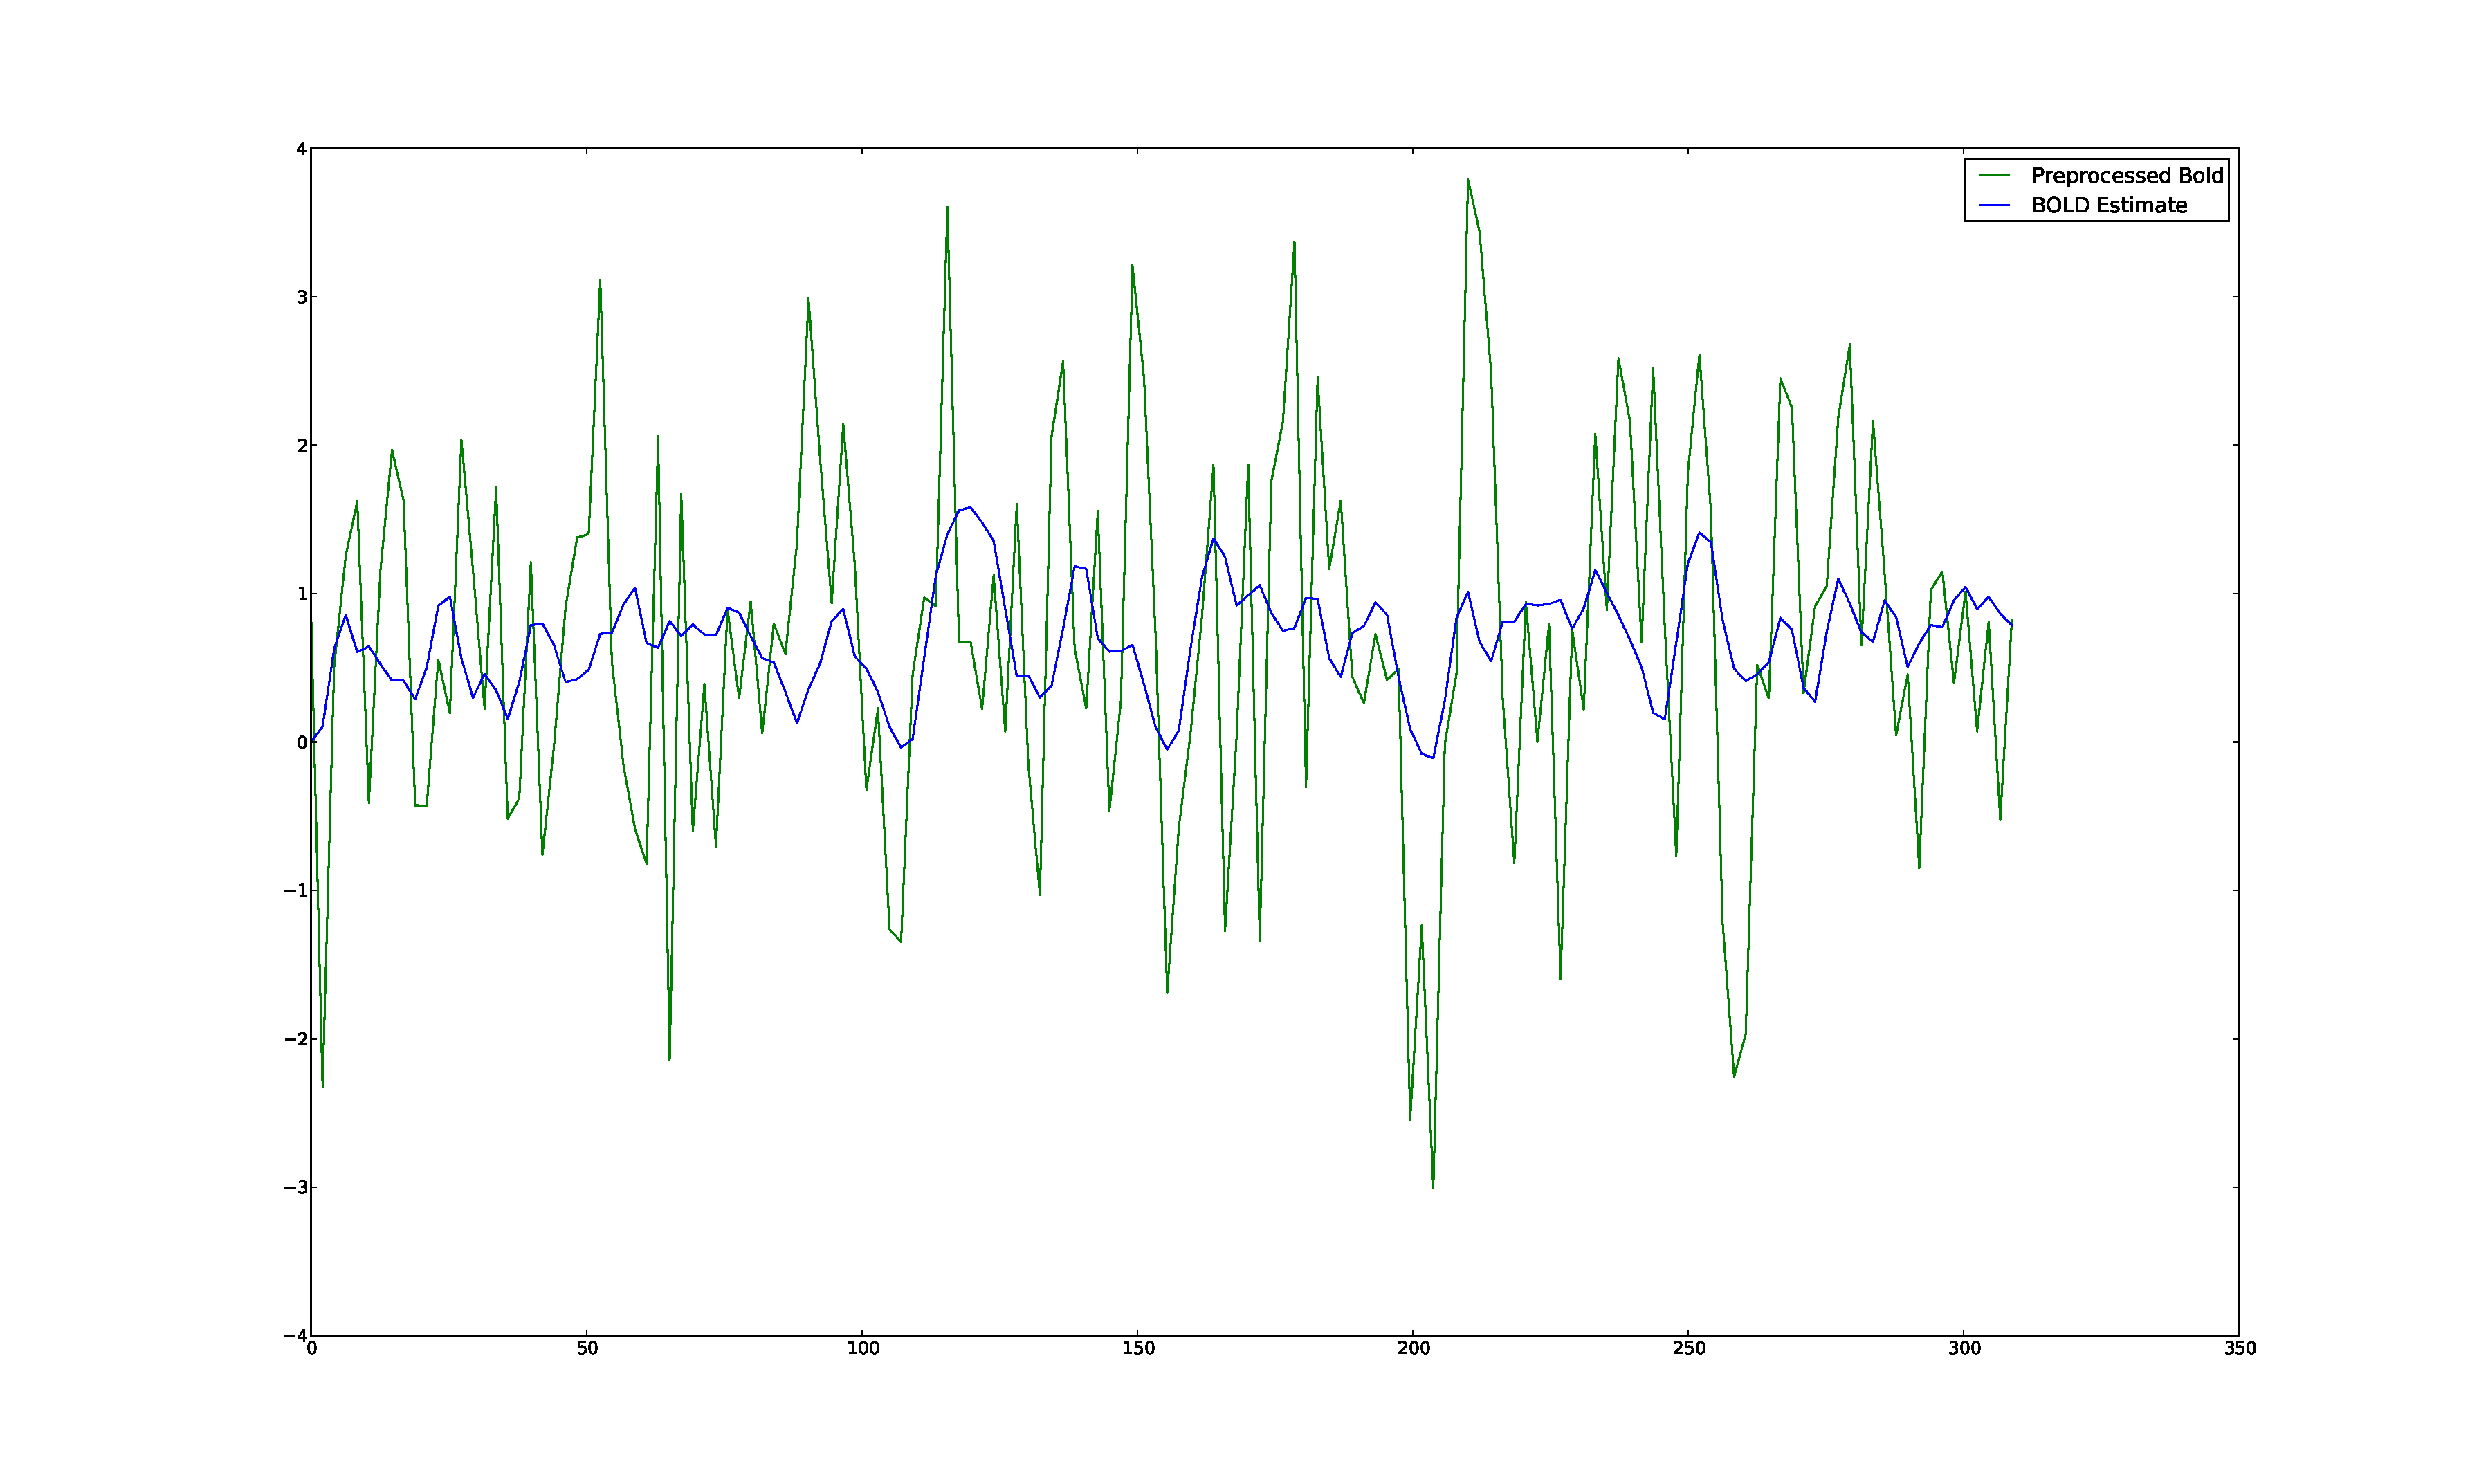
\includegraphics[clip=true,trim=5cm 1cm 4cm 1cm,width=15cm]{images/4_spm_26_15_7}}
\caption{Section 4, Estimated vs. Actual BOLD response. T-Score: $0.50$, Mutual Information: $0.06$, Residual: $0.95$. }
\label{fig:comp4}
\end{figure}

% or in original coordinates 29-9-13
\begin{figure}
\subfigure[Particle Filter]{\label{fig:comp5pfilter} 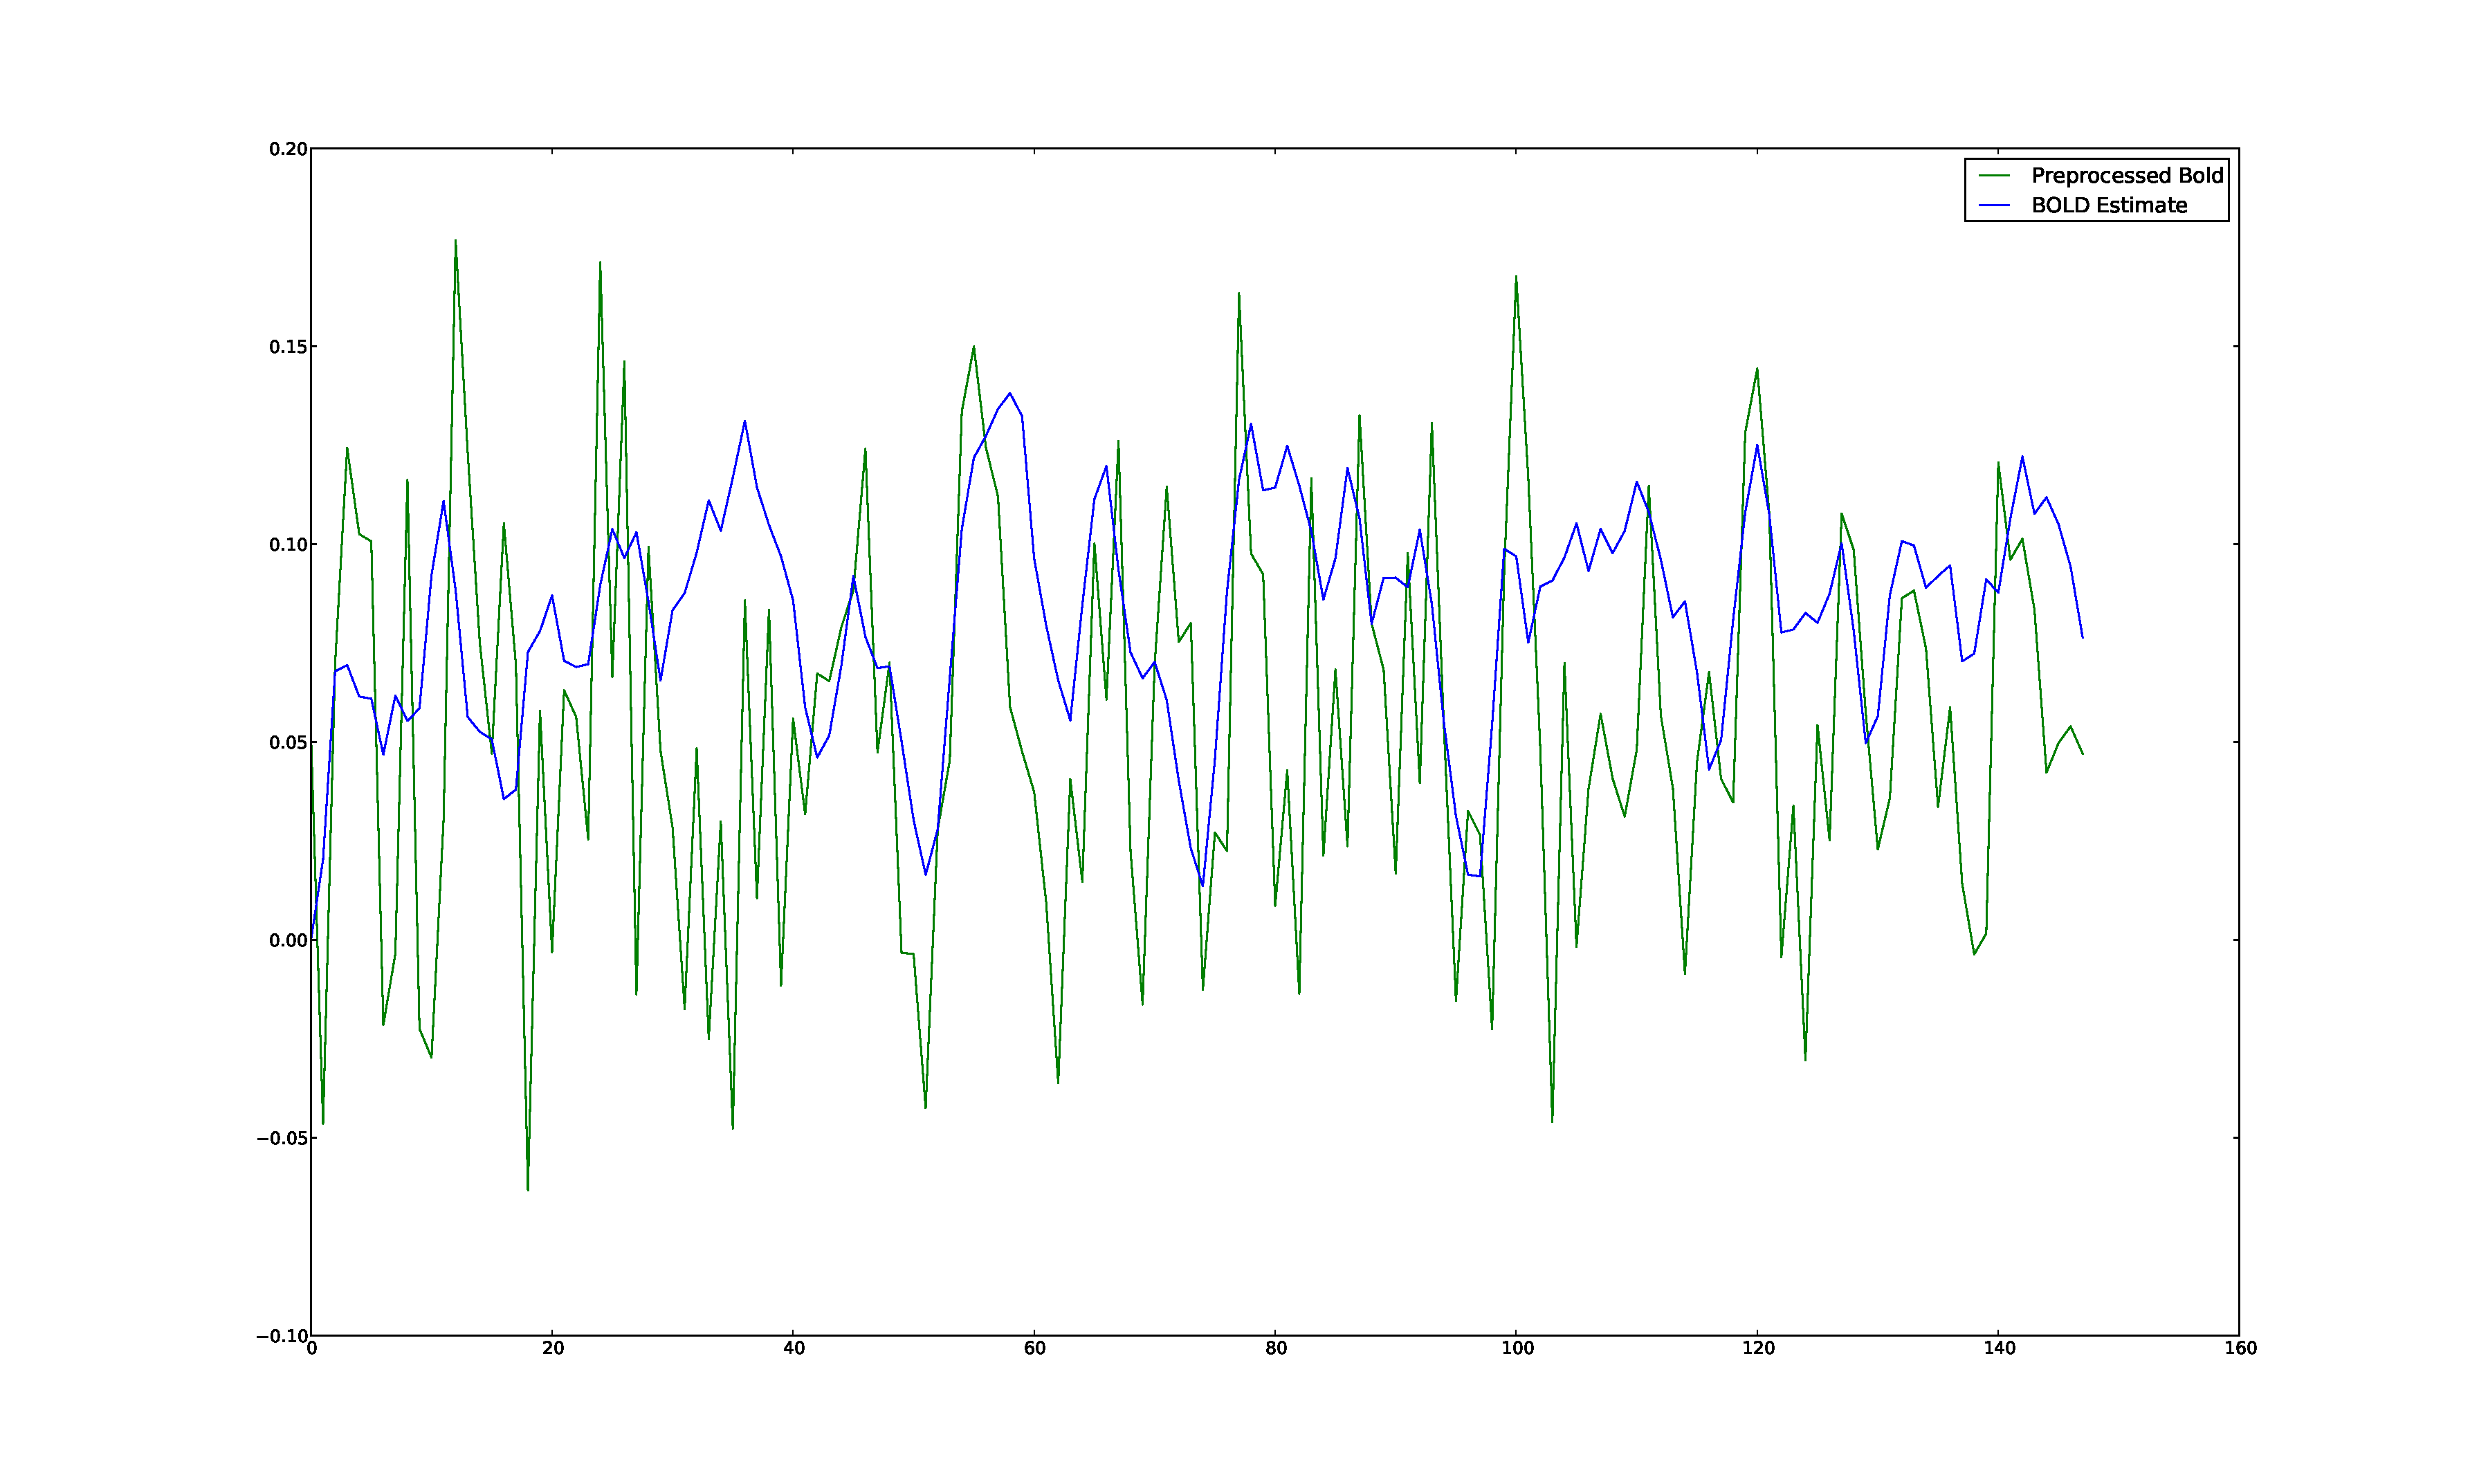
\includegraphics[clip=true,trim=5cm 1cm 4cm 1cm,width=15cm]{images/5_pfilter_29_9_13}}\\
\subfigure[SPM]{\label{fig:comp5spm} 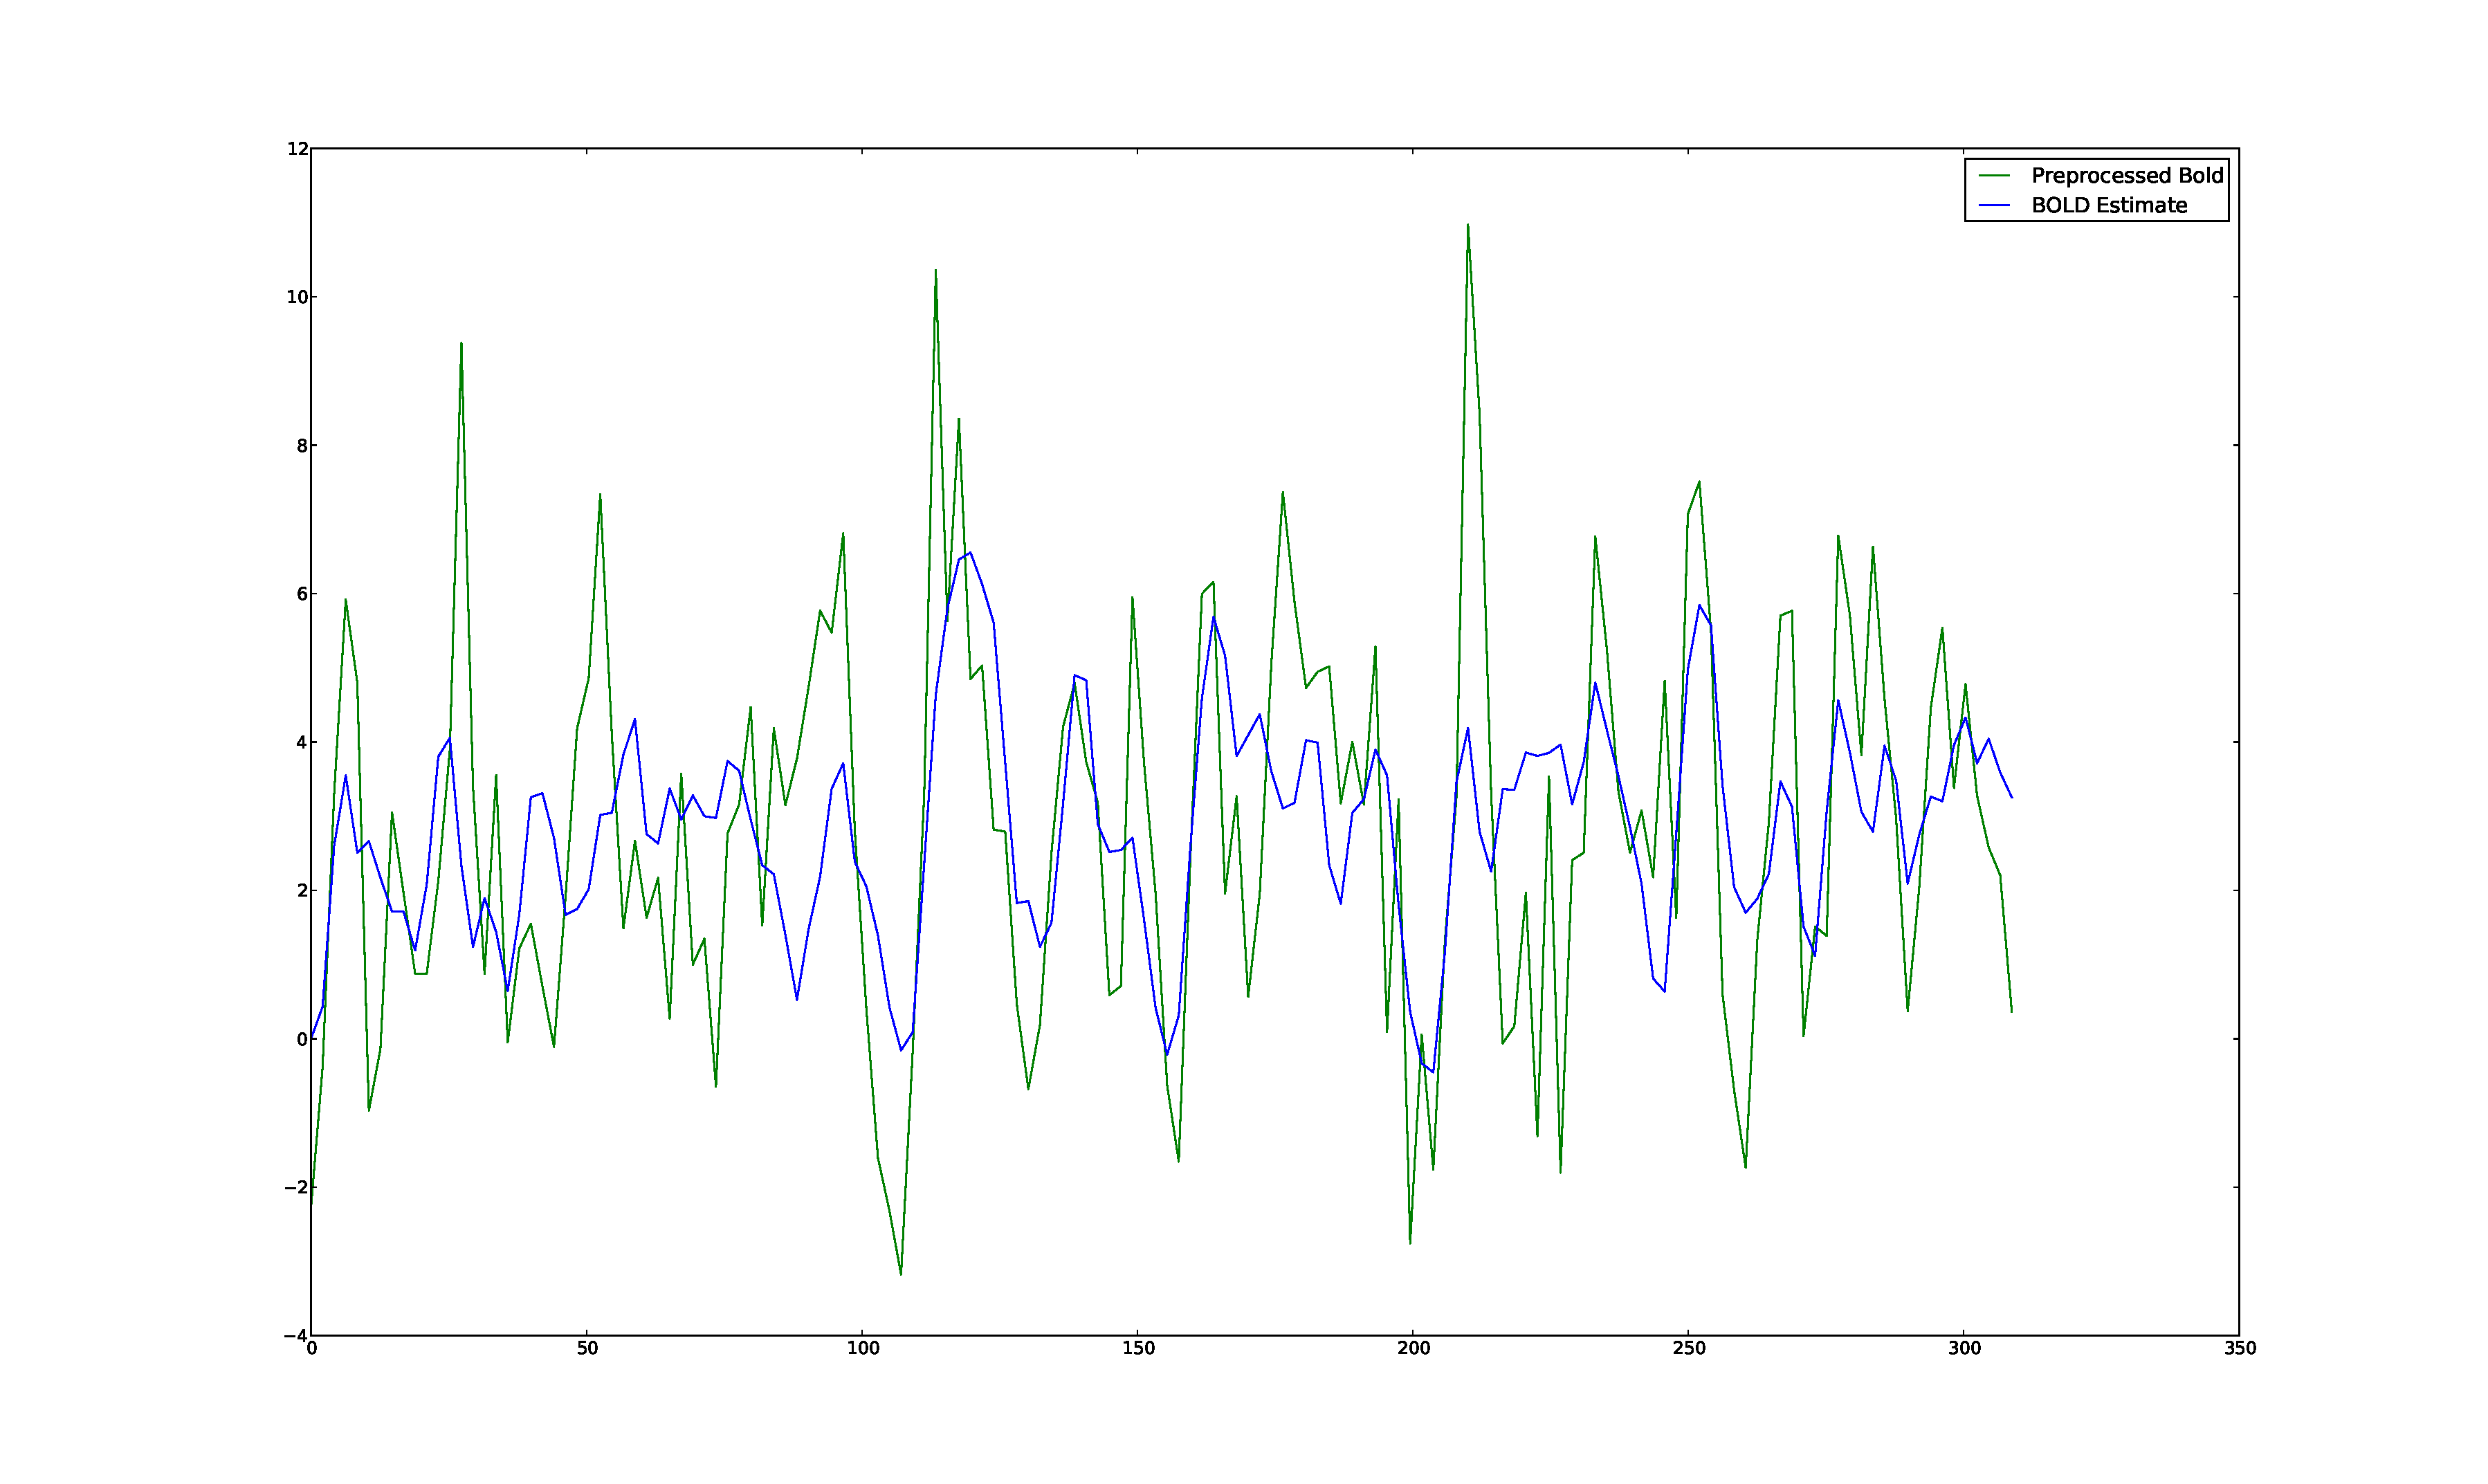
\includegraphics[clip=true,trim=5cm 1cm 4cm 1cm,width=15cm]{images/5_spm_29_9_13}}
\caption{Section 5, Estimated vs. Actual BOLD Response. T-Score: $4.17$, Mutual Information: $0.02$, Residual: $1.14$.}
%\caption{Section 5, Below threshold in both particle filter checks, but above threshold in SPM. Mutual Information of $0.0212822$, T-Value
%of $4.17399$ and $MSE$ of $1.14171$.}
\label{fig:comp5}
\end{figure}

%23-10-18 or in original coordinates 36-17-19
\begin{figure}
\subfigure[Particle Filter]{\label{fig:comp6pfilter} 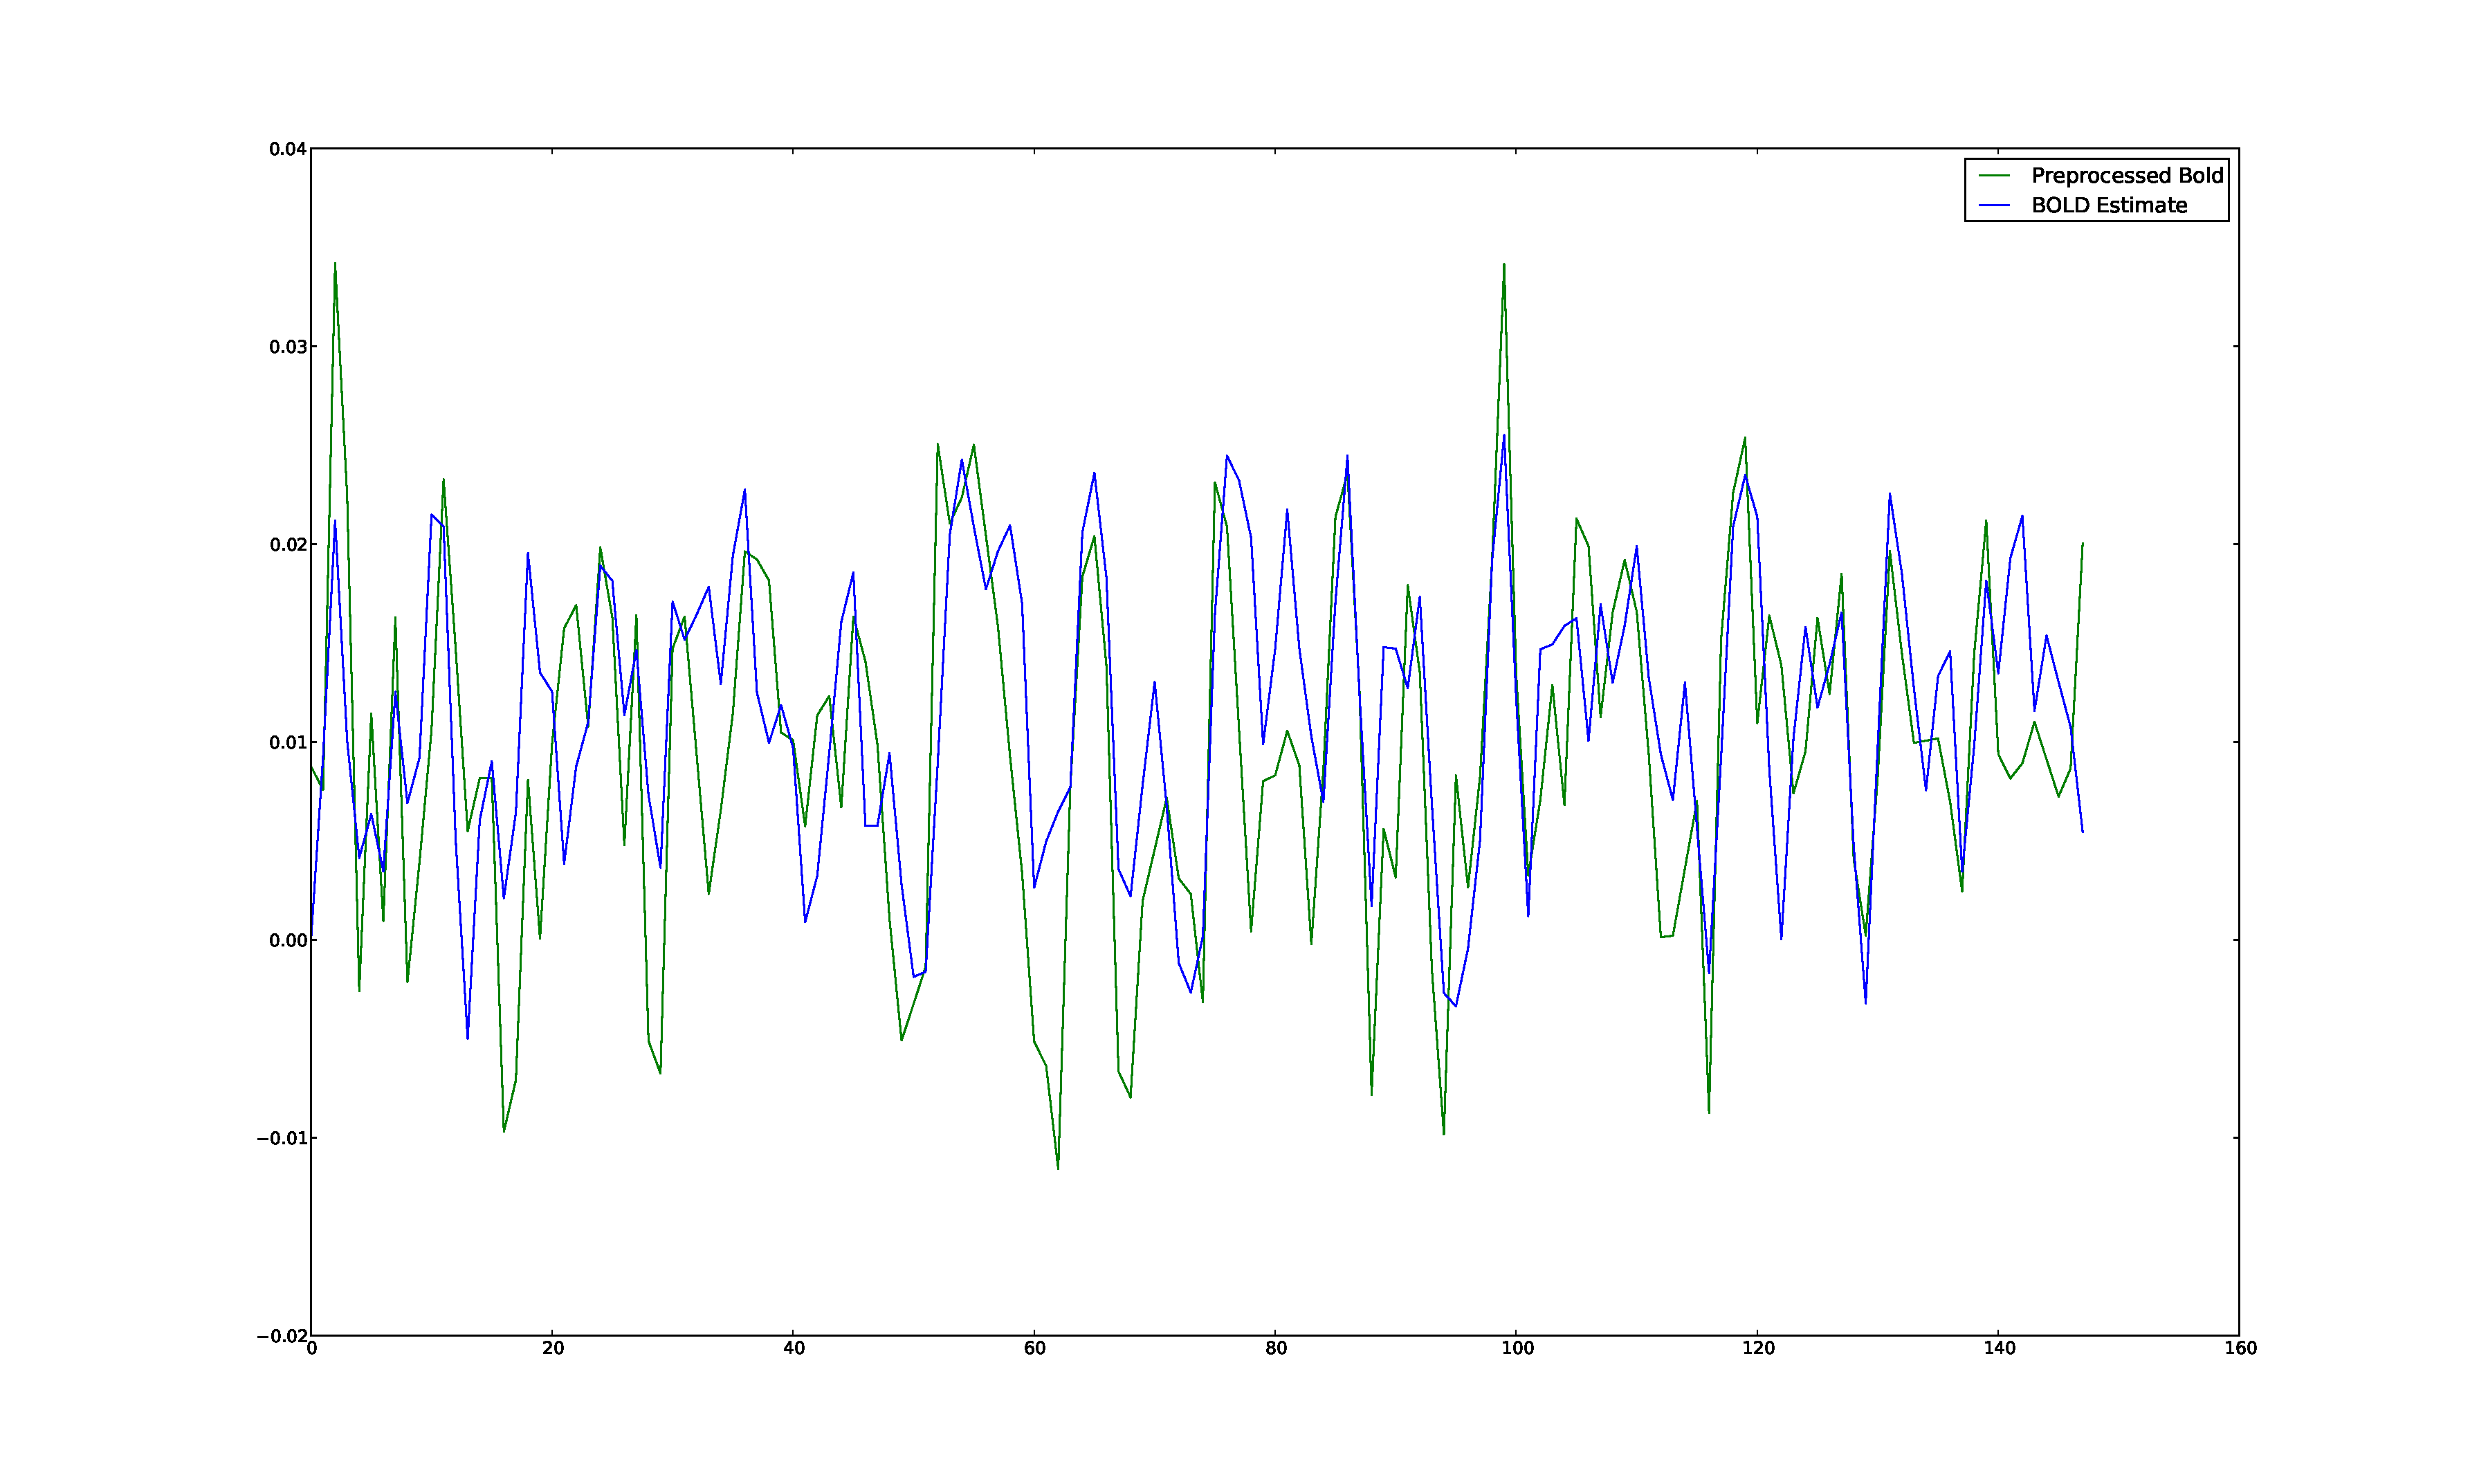
\includegraphics[clip=true,trim=5cm 1cm 4cm 1cm,width=15cm]{images/6_pfilter_36_17_19}}\\
\subfigure[SPM]{\label{fig:comp6spm} 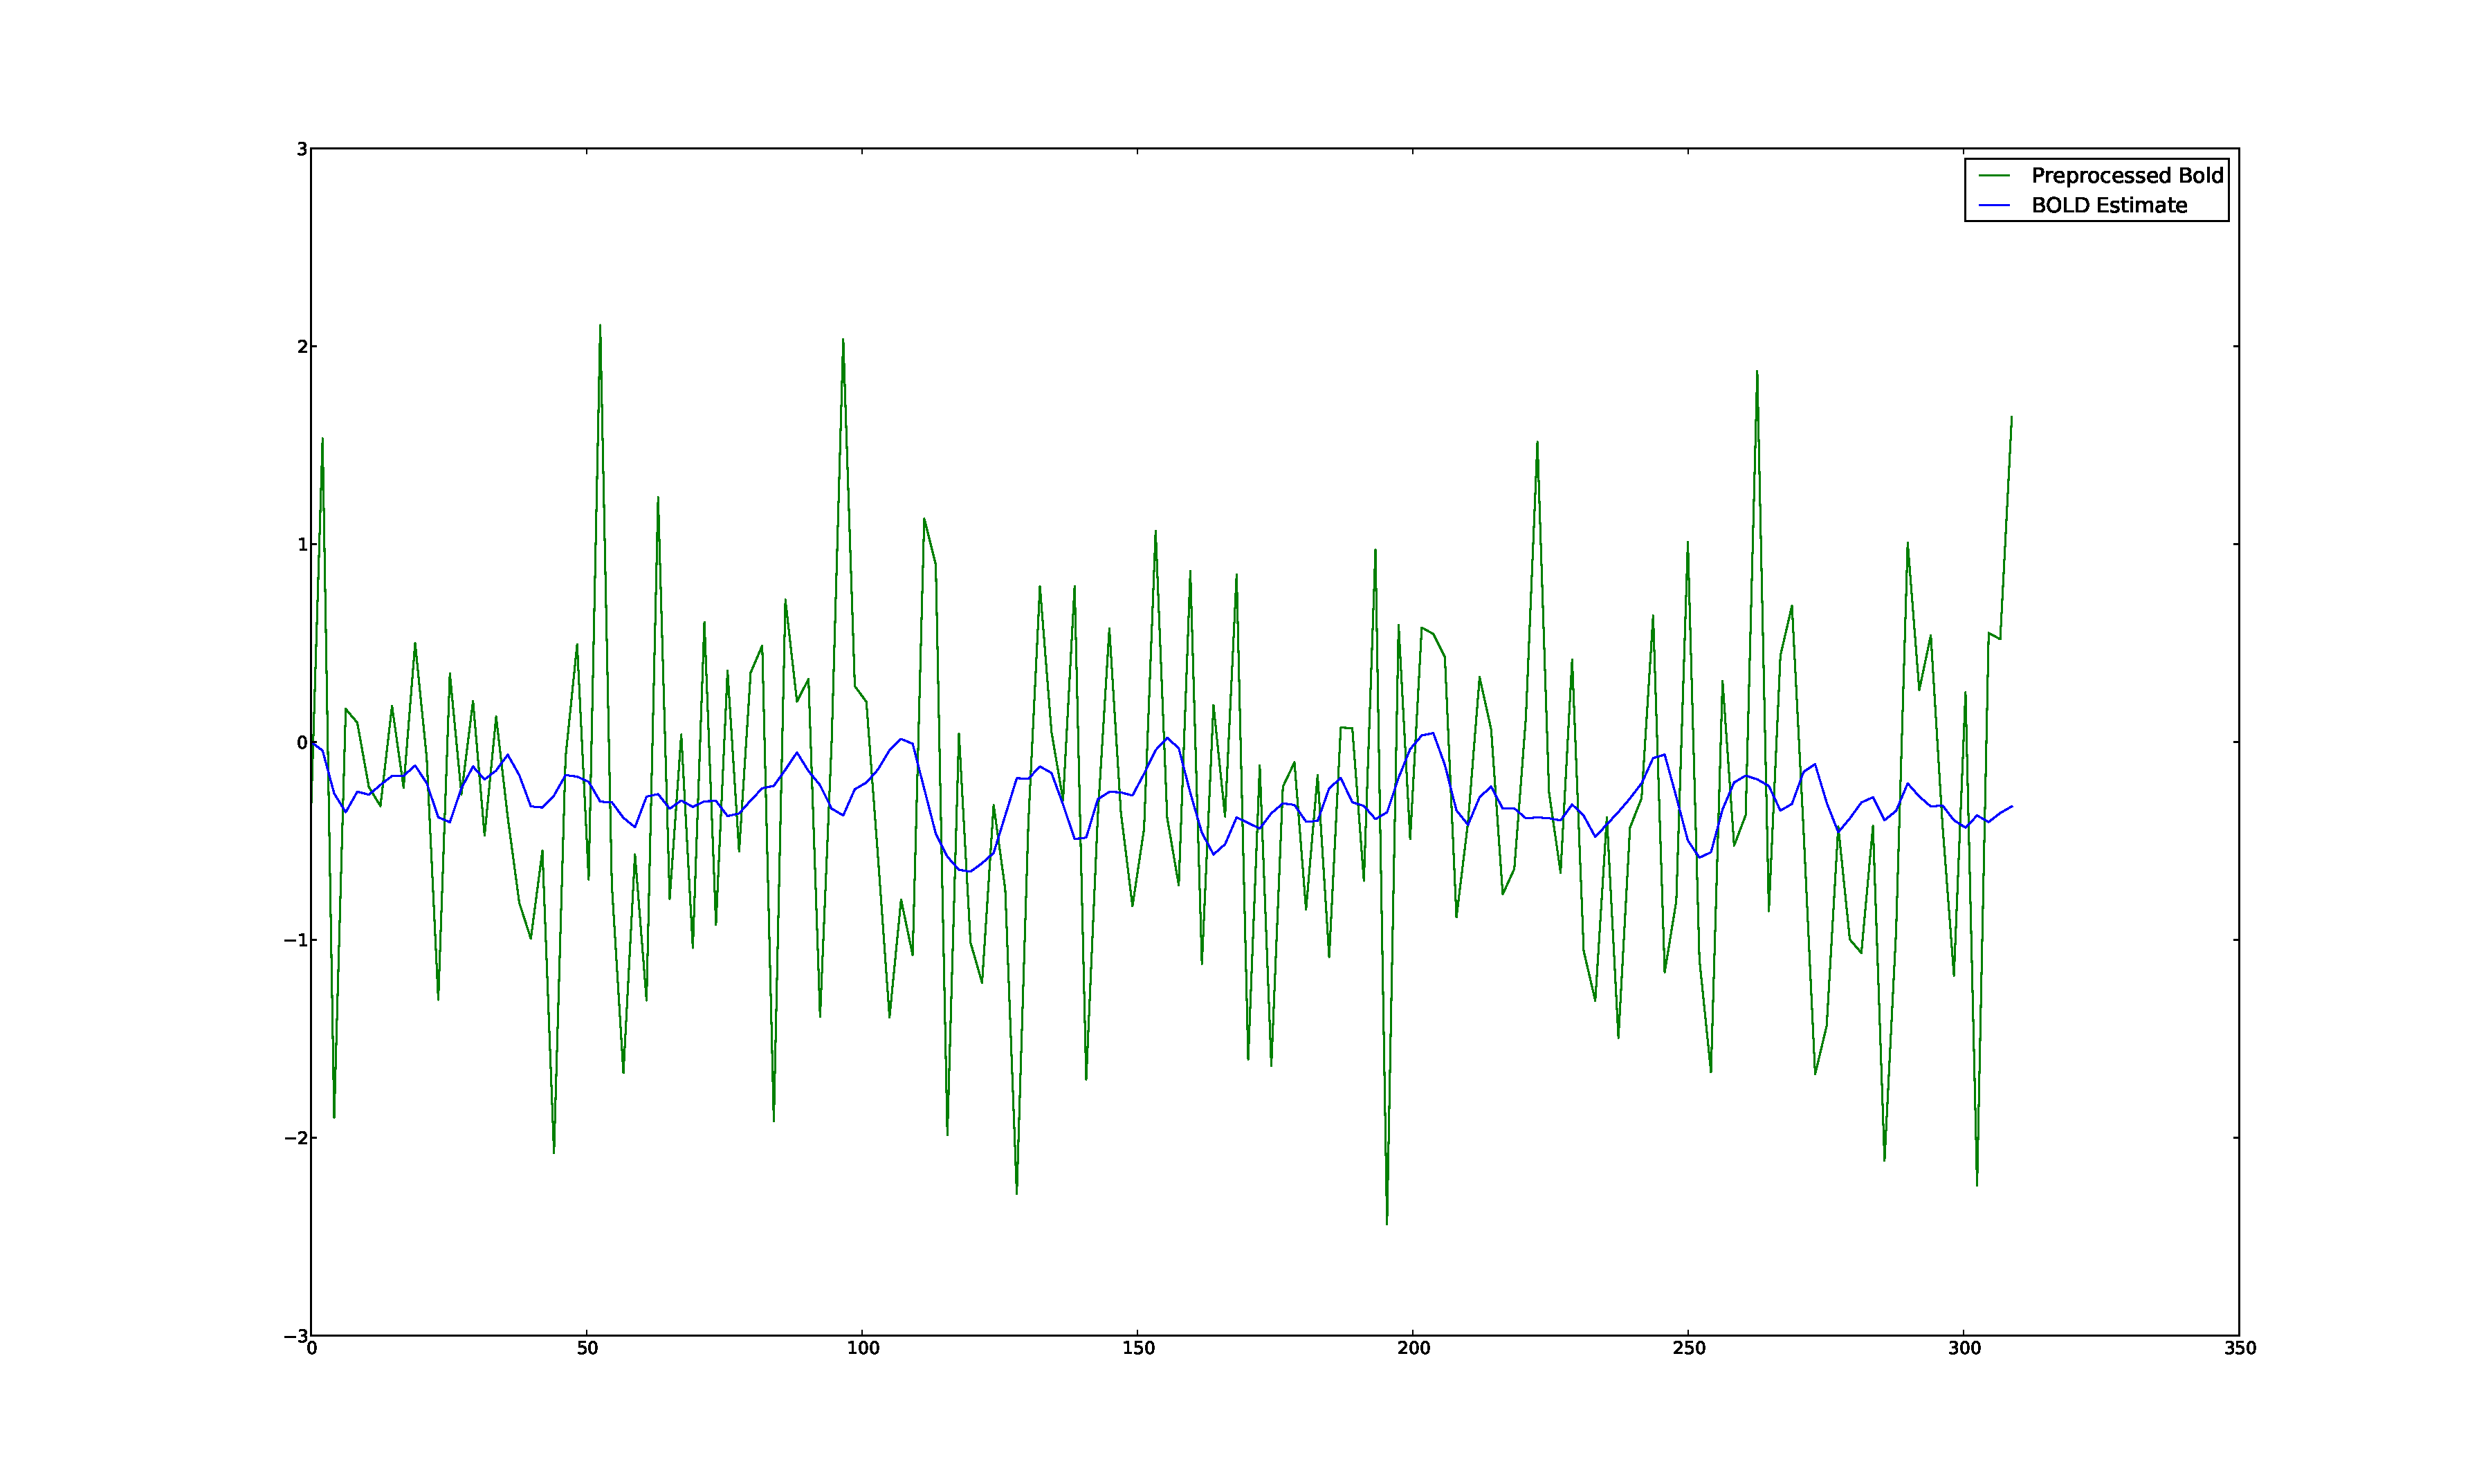
\includegraphics[clip=true,trim=5cm 1cm 4cm 1cm,width=15cm]{images/6_spm_36_17_19}}
\caption{Section 6, Estimated vs. Actual BOLD Response. T-Score: $2.49$, Mutual Information: $.34$, Residual: $0.78$.}
%\caption{Section 6, MI of $0.335504$, T Value: $2.49154$, normalized error: $0.783348$ Not visible in SPM}
\label{fig:comp6}
\end{figure}

%16-19-0 or in original coordinates 29-26-1
\begin{figure}
\subfigure[Particle Filter]{\label{fig:comp7pfilter} 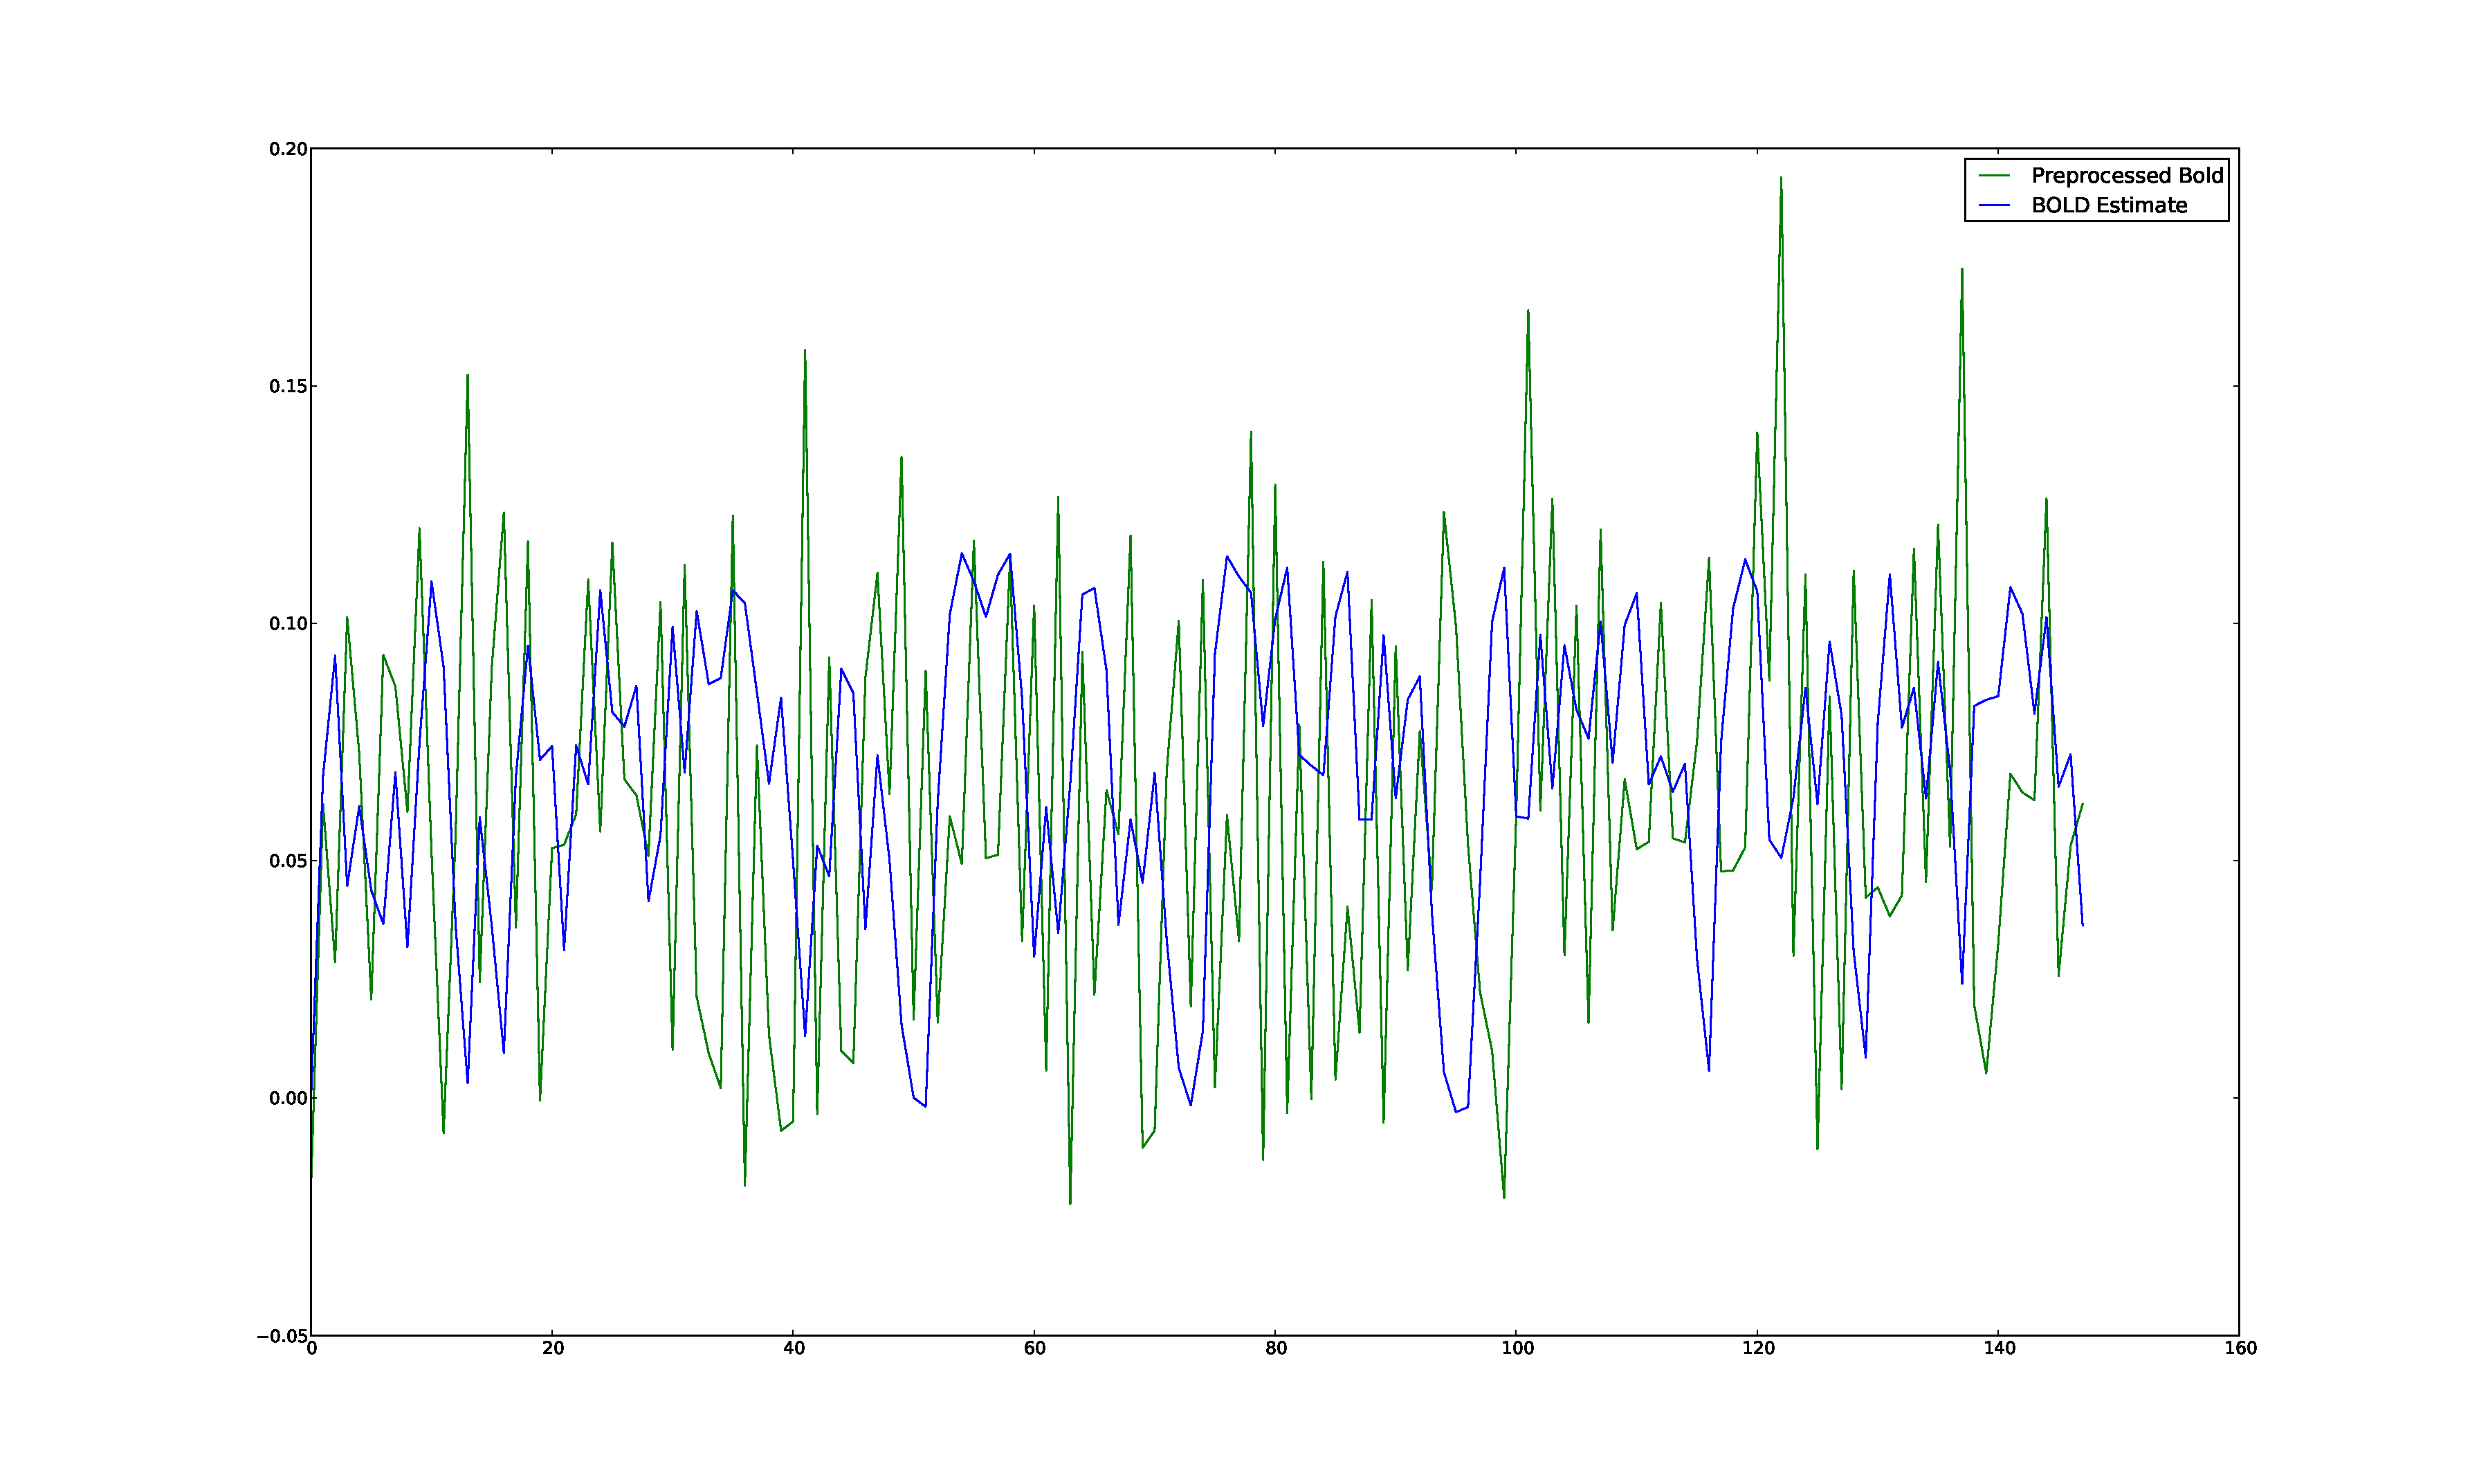
\includegraphics[clip=true,trim=5cm 1cm 4cm 1cm,width=15cm]{images/7_pfilter_29_26_1}}\\
%\subfigure[SPM]{\label{fig:comp7spm} 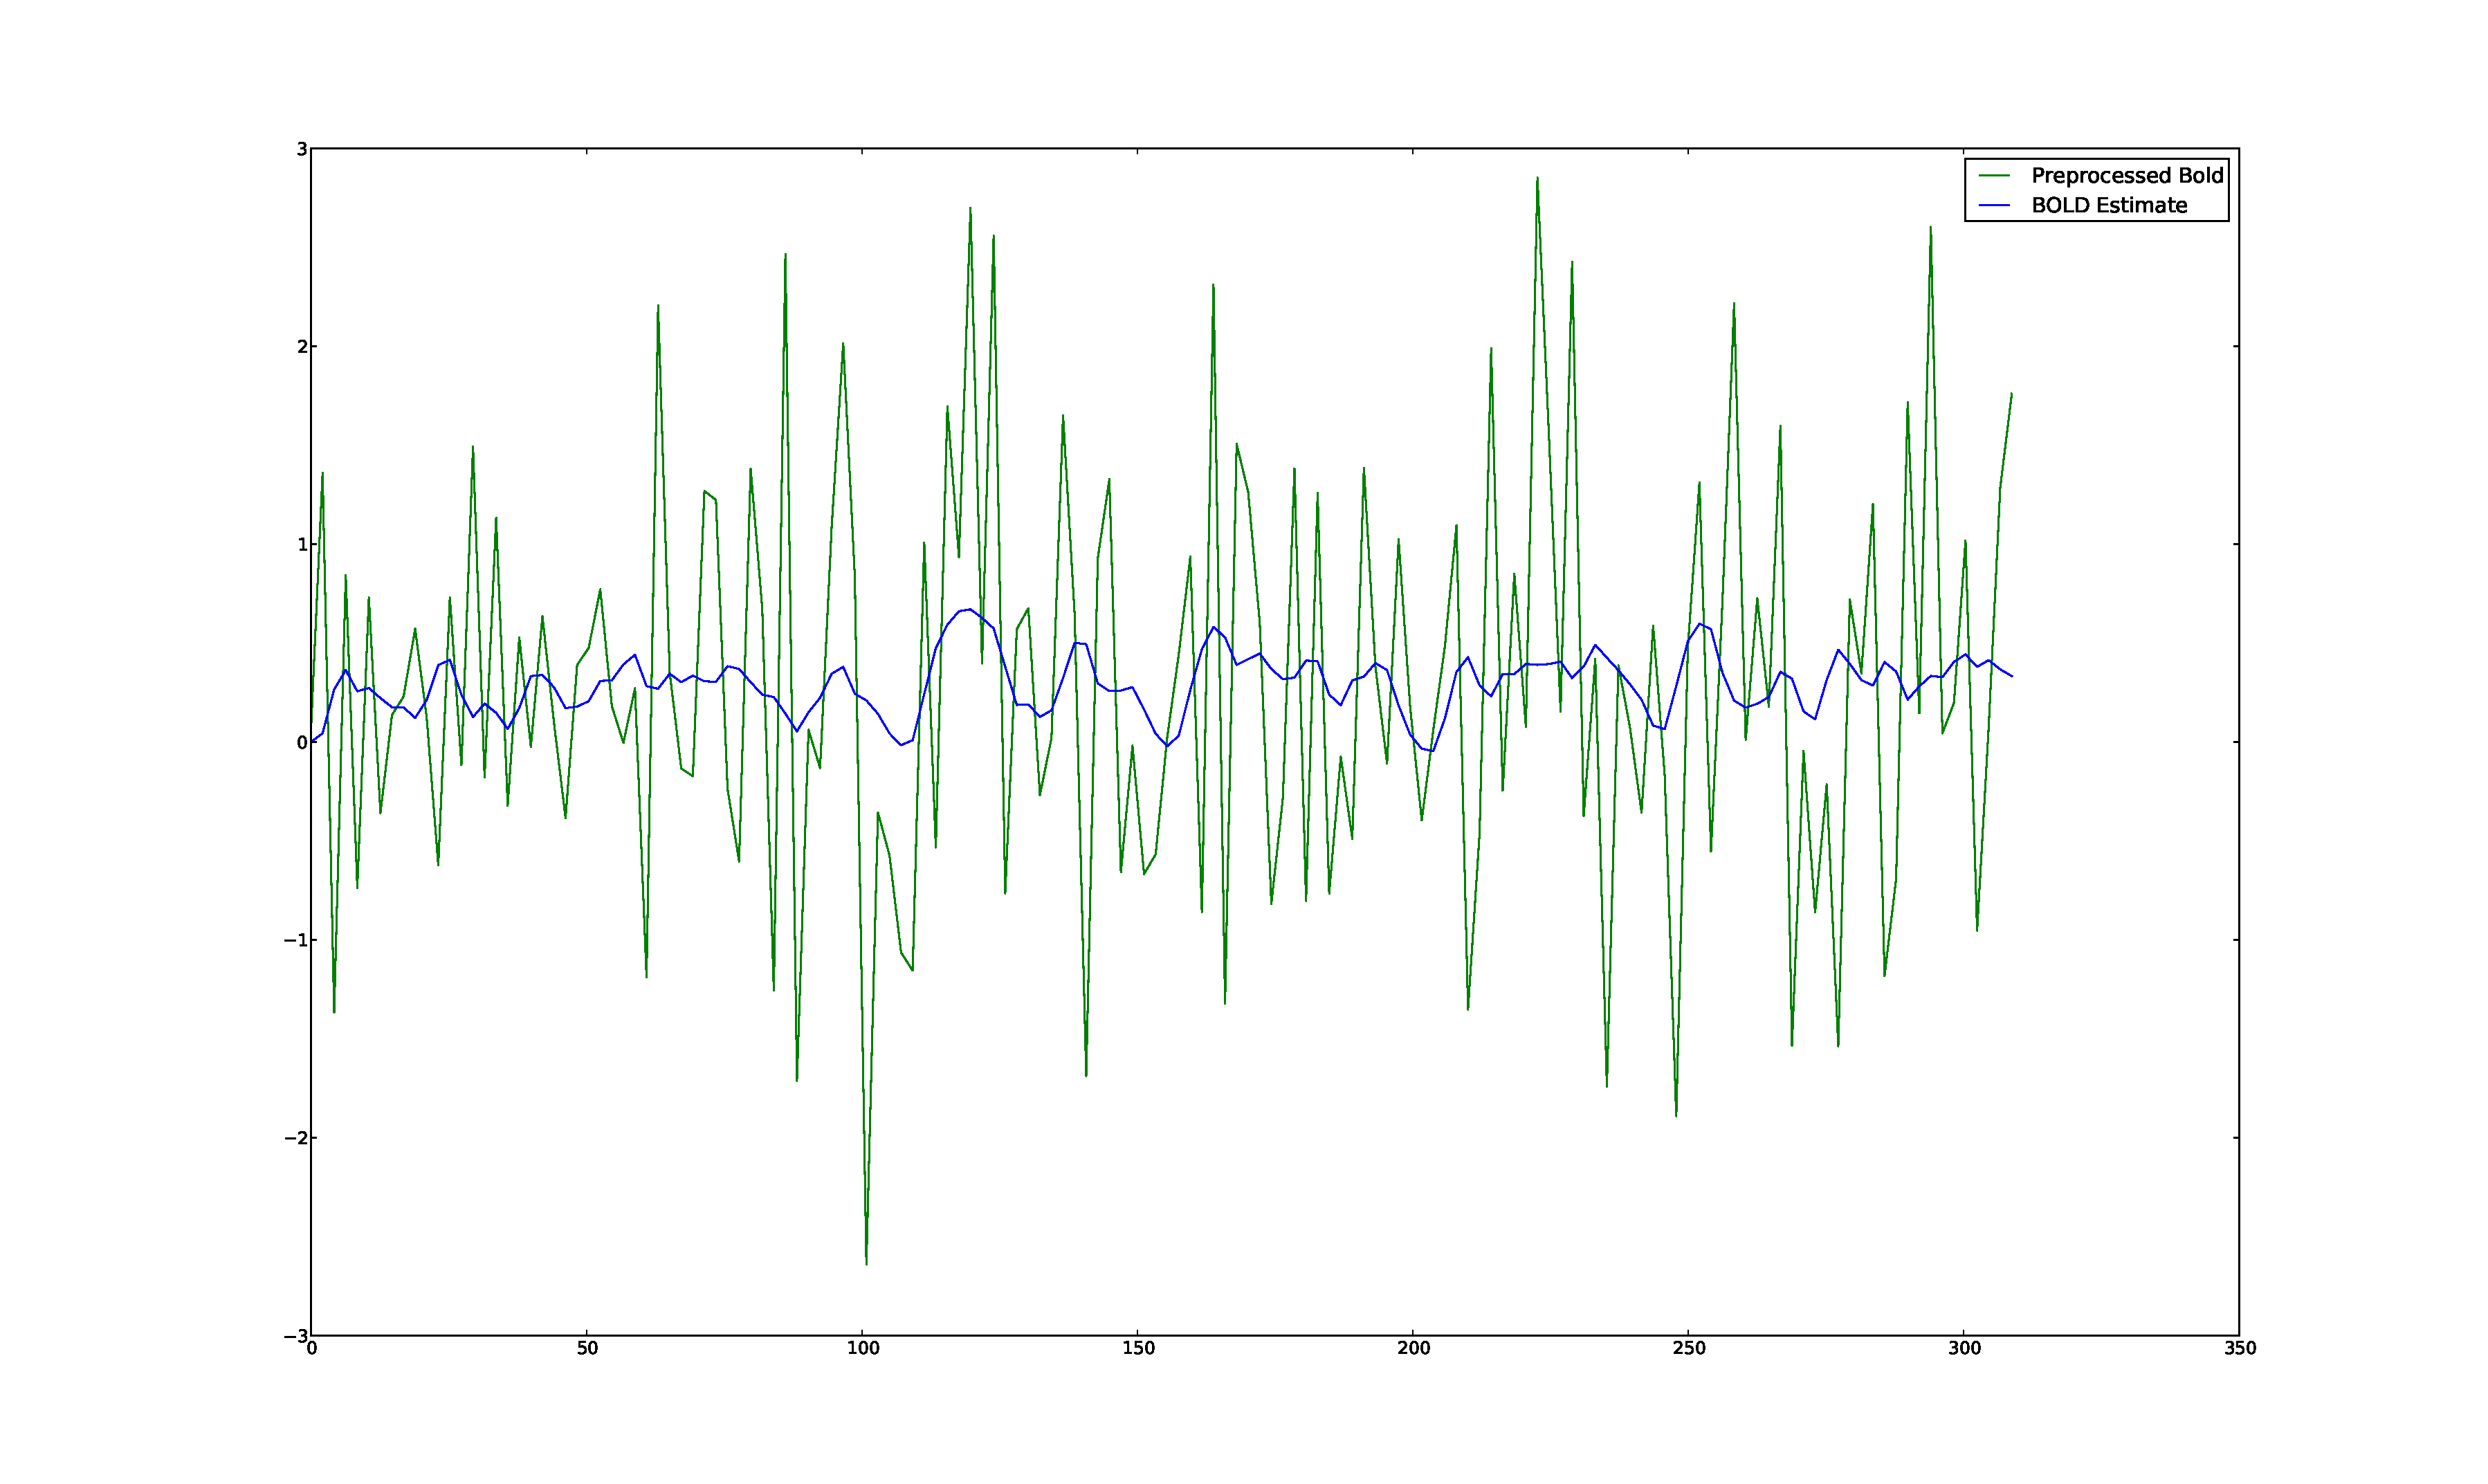
\includegraphics[clip=true,trim=5cm 1cm 4cm 1cm,width=15cm]{images/5_spm_25_34_25}}
\caption{Section 6, Estimated vs. Actual BOLD Response. T-Score: $1.32$, Mutual Information: $0.11$, Residual: $1.10$.}
%\caption{Section 7, $.1052$ in MI, $1.31534$ in SPM (which left this flat) and $1.09992$ normalized $\sqrt{MSE}$. Only visible in MI map. }
\label{fig:comp7}
\end{figure}

Voxel 6 (\autoref{fig:comp6}) is another region that is active according to both metrics used
in this work, yet was missed by SPM. The time series in \autoref{fig:comp6} shows an extremely
good fit, perhaps the best in this batch, for the particle filter. In contrast, the
fit for SPM is abysmal. In spite of the fact that several other areas around are active
as well, the smoothing seems to have completely wiped out activation in this voxel. 

Finally voxel 7 is a completely ambiguous time series. While the thresholds applied here
are empirical, this voxel is on the borderline of the thresholds for both mutual information
and the residual. The signal itself is extremely noisy, it should the voxel should be rejected.
However this case is reminiscent of the pure-noise tests performed in the previous chapter. 
This time series an extremely good example of the danger of false positives. In spite of the
fact that the signal oscillates far faster than the BOLD estimate, because of that, it is somehow
able to maintain a mutual information value of $.1052$ and a residual of just $1.09992$.
As such, a clear method of detecting these sorts of regions is necessary if the results
of the particle filter algorithm are toe be trusted. 

\section{Parameter Estimates}
\label{sec:Real Data Parameter Estimates}
Although the parameters are not uniquely identifiable by a single time-series, that
does not mean estimating them is not without benefit. The parameters still contain useful
information about the system. Additionally, as an aggregate they form a distribution of
the feasible parameters parameters for a particular patient. Therefore 
\autoref{fig:pmap0} through \autoref{fig:pmap6}
contain the parameter maps for the system and \autoref{fig:realhist} is a histogram across all voxels
for which the mutual information was greater than $.15$. As before, the threshold is not
scientifically derived, yet in tests this threshold provided a decent balance to remove most
of the questionably active voxels in the system. 

\begin{figure}[H]
\centering
\subfigure{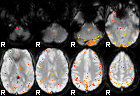
\includegraphics[width=13cm]{images/pmap0}}
\subfigure{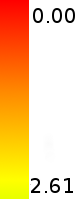
\includegraphics[scale=.5]{images/pscale_00}}
\caption{$\tau_0$ Estimates}
\label{fig:pmap0}
\end{figure}

\begin{figure}[H]
\centering
\subfigure{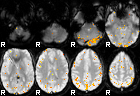
\includegraphics[width=13cm]{images/pmap1}}
\subfigure{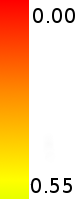
\includegraphics[scale=.5]{images/pscale_01}}
\caption{$\alpha$ Estimates}
\label{fig:pmap1}
\end{figure}

\begin{figure}[H]
\centering
\subfigure{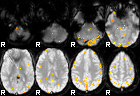
\includegraphics[width=13cm]{images/pmap2}}
\subfigure{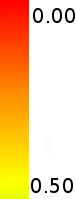
\includegraphics[scale=.5]{images/pscale_02}}
\caption{$E_0$ Estimates}
\label{fig:pmap2}
\end{figure}

\begin{figure}[H]
\centering
\subfigure{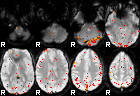
\includegraphics[width=13cm]{images/pmap3}}
\subfigure{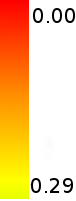
\includegraphics[scale=.5]{images/pscale_03}}
\caption{$V_0$ Estimates}
\label{fig:pmap3}
\end{figure}

\begin{figure}[H]
\centering
\subfigure{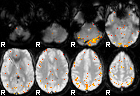
\includegraphics[width=13cm]{images/pmap4}}
\subfigure{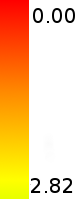
\includegraphics[scale=.5]{images/pscale_04}}
\caption{$\tau_f$ Estimates}
\label{fig:pmap4}
\end{figure}

\begin{figure}[H]
\centering
\subfigure{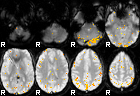
\includegraphics[width=13cm]{images/pmap5}}
\subfigure{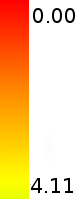
\includegraphics[scale=.5]{images/pscale_05}}
\caption{$\tau_s$ Estimates}
\label{fig:pmap5}
\end{figure}

\begin{figure}[H]
\centering
\subfigure{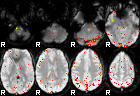
\includegraphics[width=13cm]{images/pmap6}}
\subfigure{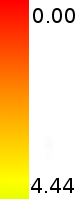
\includegraphics[scale=.5]{images/pscale_06}}
\caption{$\epsilon$ Estimates}
\label{fig:pmap6}
\end{figure}

Regions with poor fit cannot have reliable parameter estimates because the input did not meaningfully
correlate input with output. Therefore before creating the maps,
each parameters map was masked to regions with mutual information greater than $.15$. I chose mutual
information over the residual because in the maps comparing regression fitness, the mutual information
maps had more coherency and less randomness. Additionally, in the single voxel tests (\autoref{sec:SingleVoxelReview}) 
there was more separation between the no signal case and the signal case than there was in the 
residual metric. 

\begin{figure}
\centering
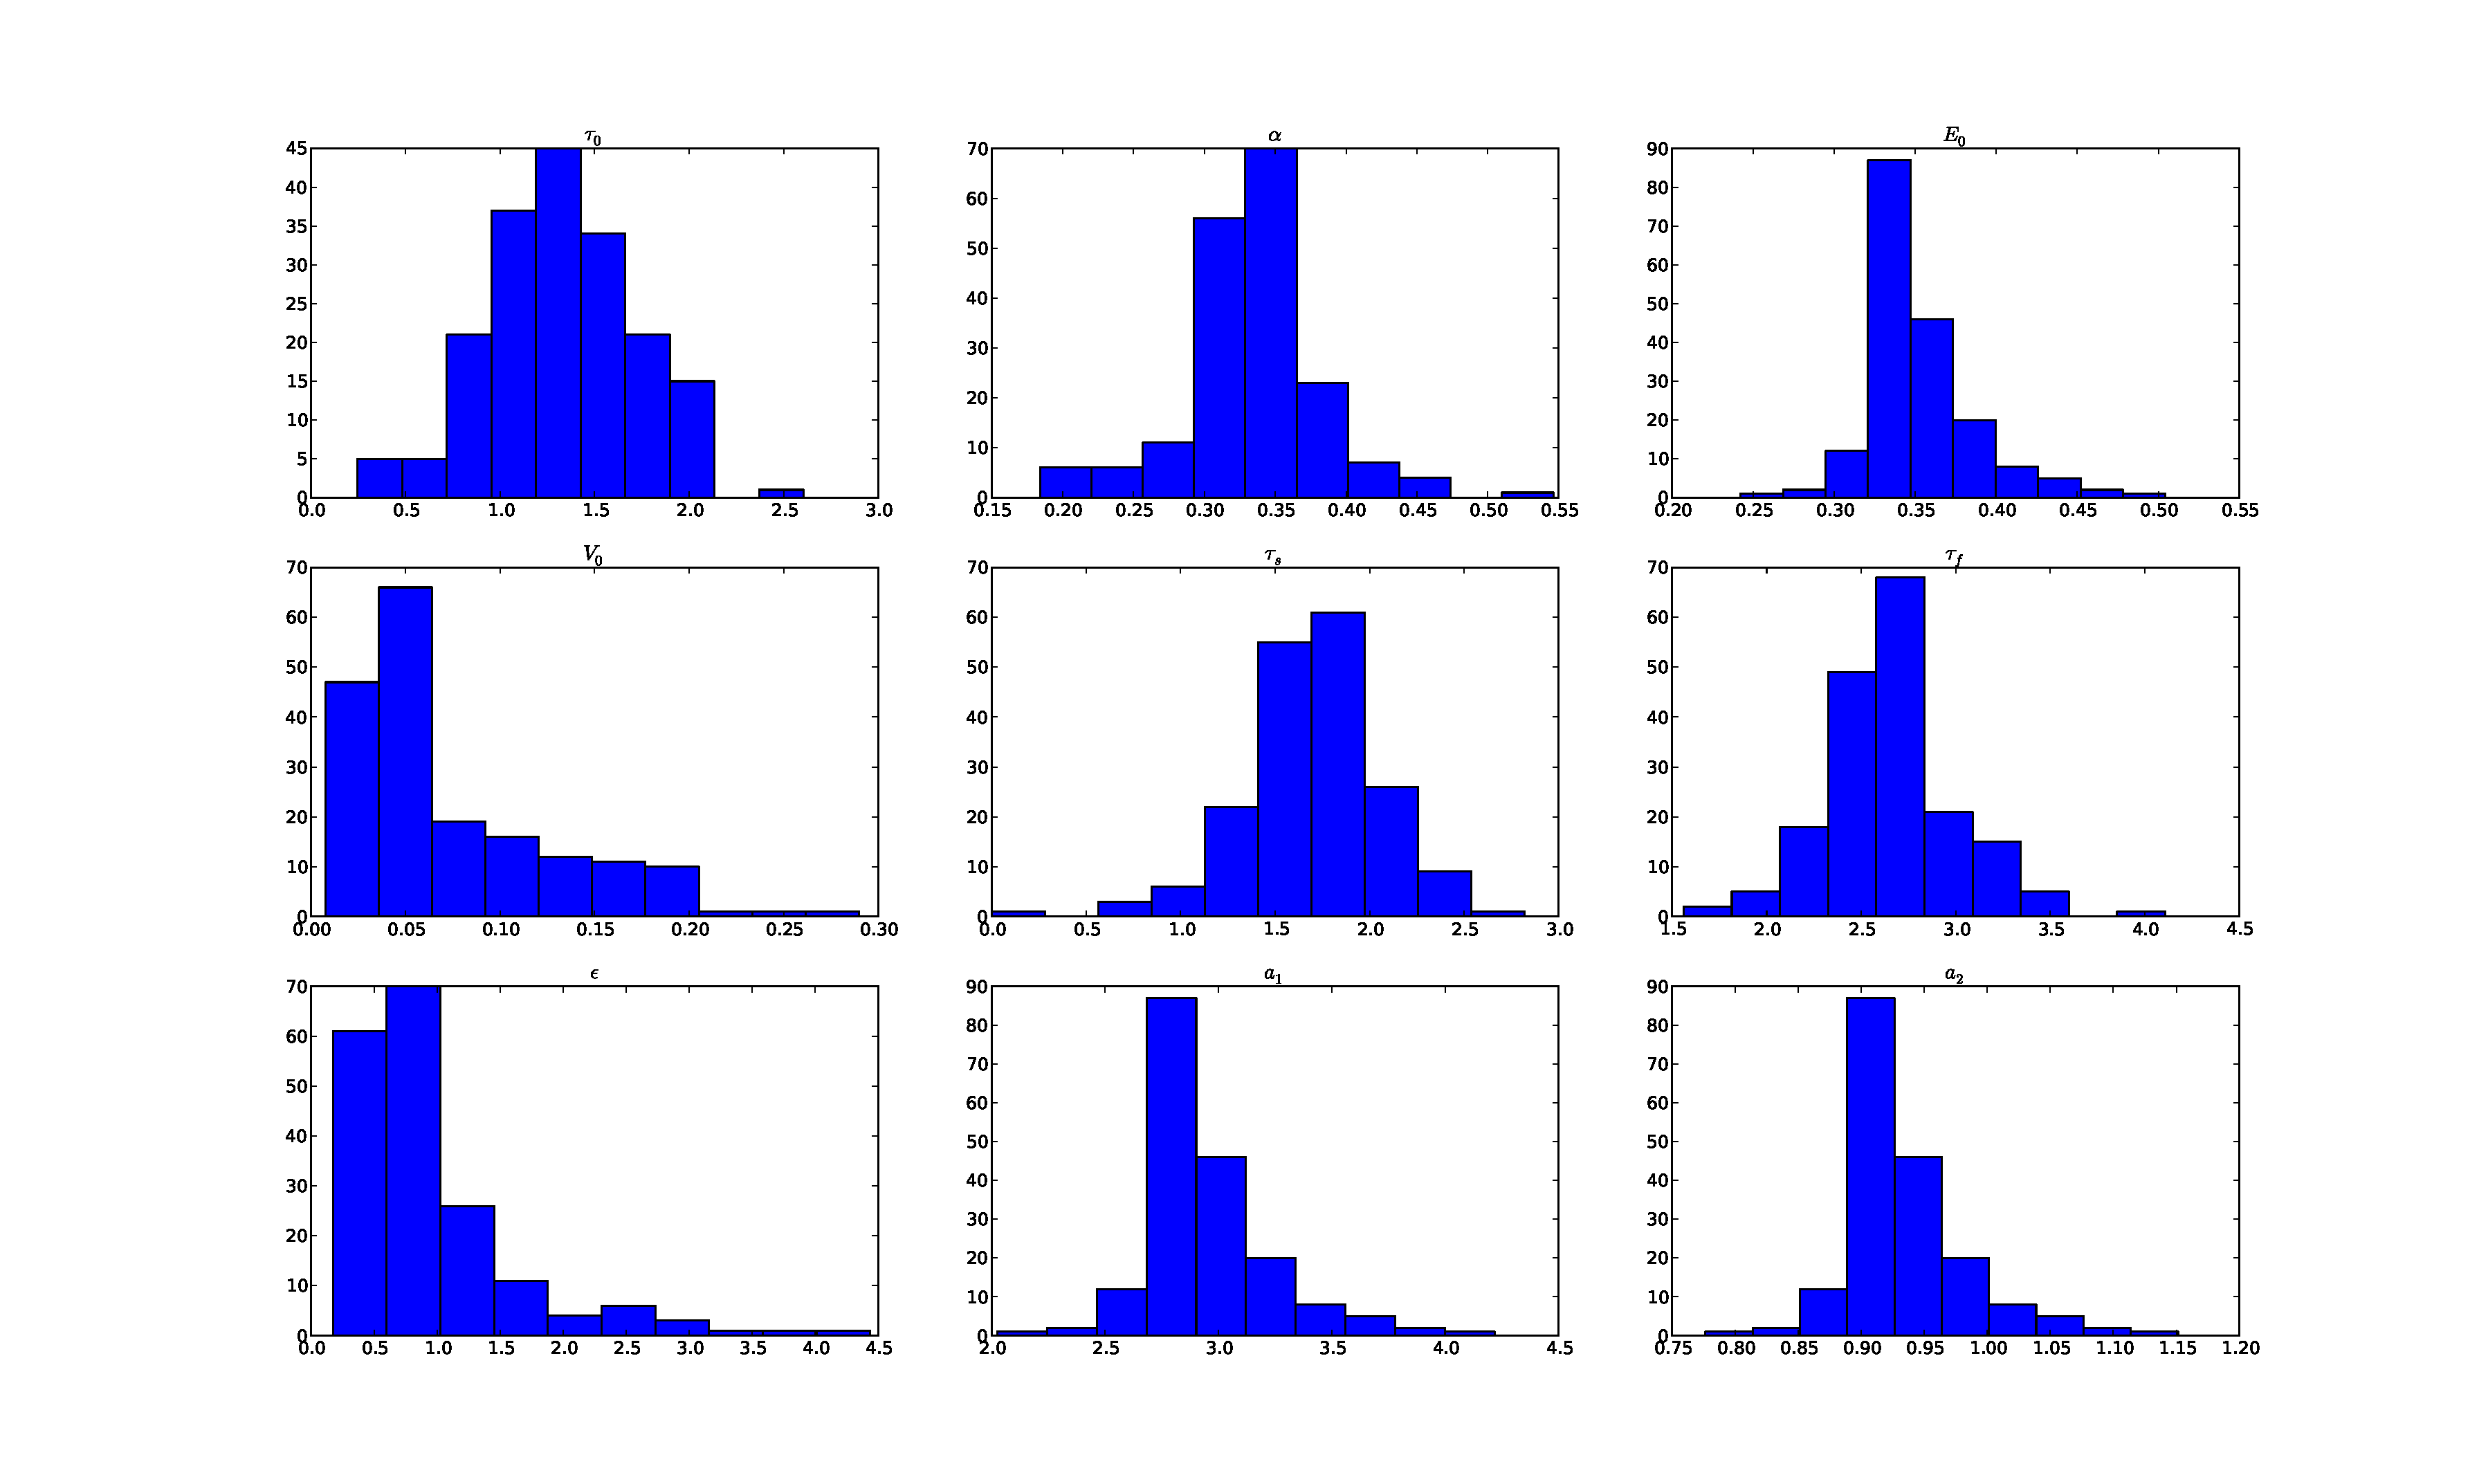
\includegraphics[clip=truew,trim=8cm 4cm 8cm 4cm,width=16cm]{images/realhist}
\caption{Histogram of parameters in active regions ($M.I. > .15$).}
\label{fig:realhist}
\end{figure}

The parameter maps show consistency parameter across active regions, however, 
the histogram of parameter estimates across all regions with $M.I. > .15$ is the
more interesting result (\autoref{fig:realhist}). 

\section{Discussion}
From the maps generated, the similarities to SPM8's results are encouraging. At the 
very least the output of the particle filter seems to meet the quality of SPM. The normalization
of the residual is certainly necessary. Although there is no hard threshold on the 
normalized residual, it would appear that the normalization is providing a reasonable
ordering of regression quality. Mutual information also shows promising results.
Many of the differences between SPM and the particle filter seem to be driven
more by the pre-processing methods than the regression methd. The reason for 
SPM applying such extrensive smoothing is to combat false positives. While this is
extremely important, regions such as \autoref{fig:comp6} show the problem with doing 
so. In all, the particle filter method does very good job of estimating parameters that
fit the measurements; and at the very least this method is a workable, albiet
computationally intensive, alternative to SPM. 
